\chapter{\VBFHBB\, Analysis}\label{c:K}

	After comparing the base constituents of the \VBFHBB\, event between the offline and HLT level and finding them to be similar in behaviour, the specific objects that make up a \VBFHBB\, event can be studied and compared. In this section, the events were required to pass all cuts discussed in Section \ref{es:as} and the designation of the jets as $b_i$, $j_i$ is highlighted in that section.


\section{Cutflow}

	Prior to investigating the core kinematic variables and the more complex kinematic variables used for the Boosted Decision Tree training (Appendix \ref{a:bdt}), the event cutflow for both the Monte-Carlo and real data should be studied to highlight any differences between the event counts. The event counts are given in Table \ref{t:cutflow}, and the ratio of the events is shown in Figures \ref{f:cutflowD} and \ref{f:cutflowMC}.

	\begin{table}[h]
		\caption{Cutflow for the \textit{two-central} \VBFHBB\, events as described in Section \ref{es:as}. The cutflows are given for the online and offline channels in both data and Monte-Carlo along with the percentage of original events.}
		\label{t:cutflow}
		\medskip
		\centering
		\begin{tabular}{c|c|c|c|c}\toprule
			Cut & MC Offline & MC Online & Data Offline & Data Online \\\midrule
			Clean Events & 6229.48 & 6229.48 & 150611000 & 150611000 \\
			Trigger & 6229.48 & 6229.48 & 6679390 &  6679390 \\
			$\geq2$ \textit{loose} \bjets & 503.552  & 467.146 & 2275760 &  2932620 \\
			$\geq2$ light-jets & 483.499  & 417.845 & 2189700 &  2671280 \\
			\textit{Tight} \bjet\, requirement & 330.962  & 288.806 & 1490320 &   1640290 \\
			Forward jet requirement & 51.843   & 40.8484 & 1186610 &  958414  \\
			\ptbb$>160$GeV & 32.7426  & 26.7038 & 309454  &  259411  \\
			\bottomrule
		\end{tabular}
	\end{table}

	\subsection{Monte-Carlo}
		\begin{figure}[h]
			\centering
			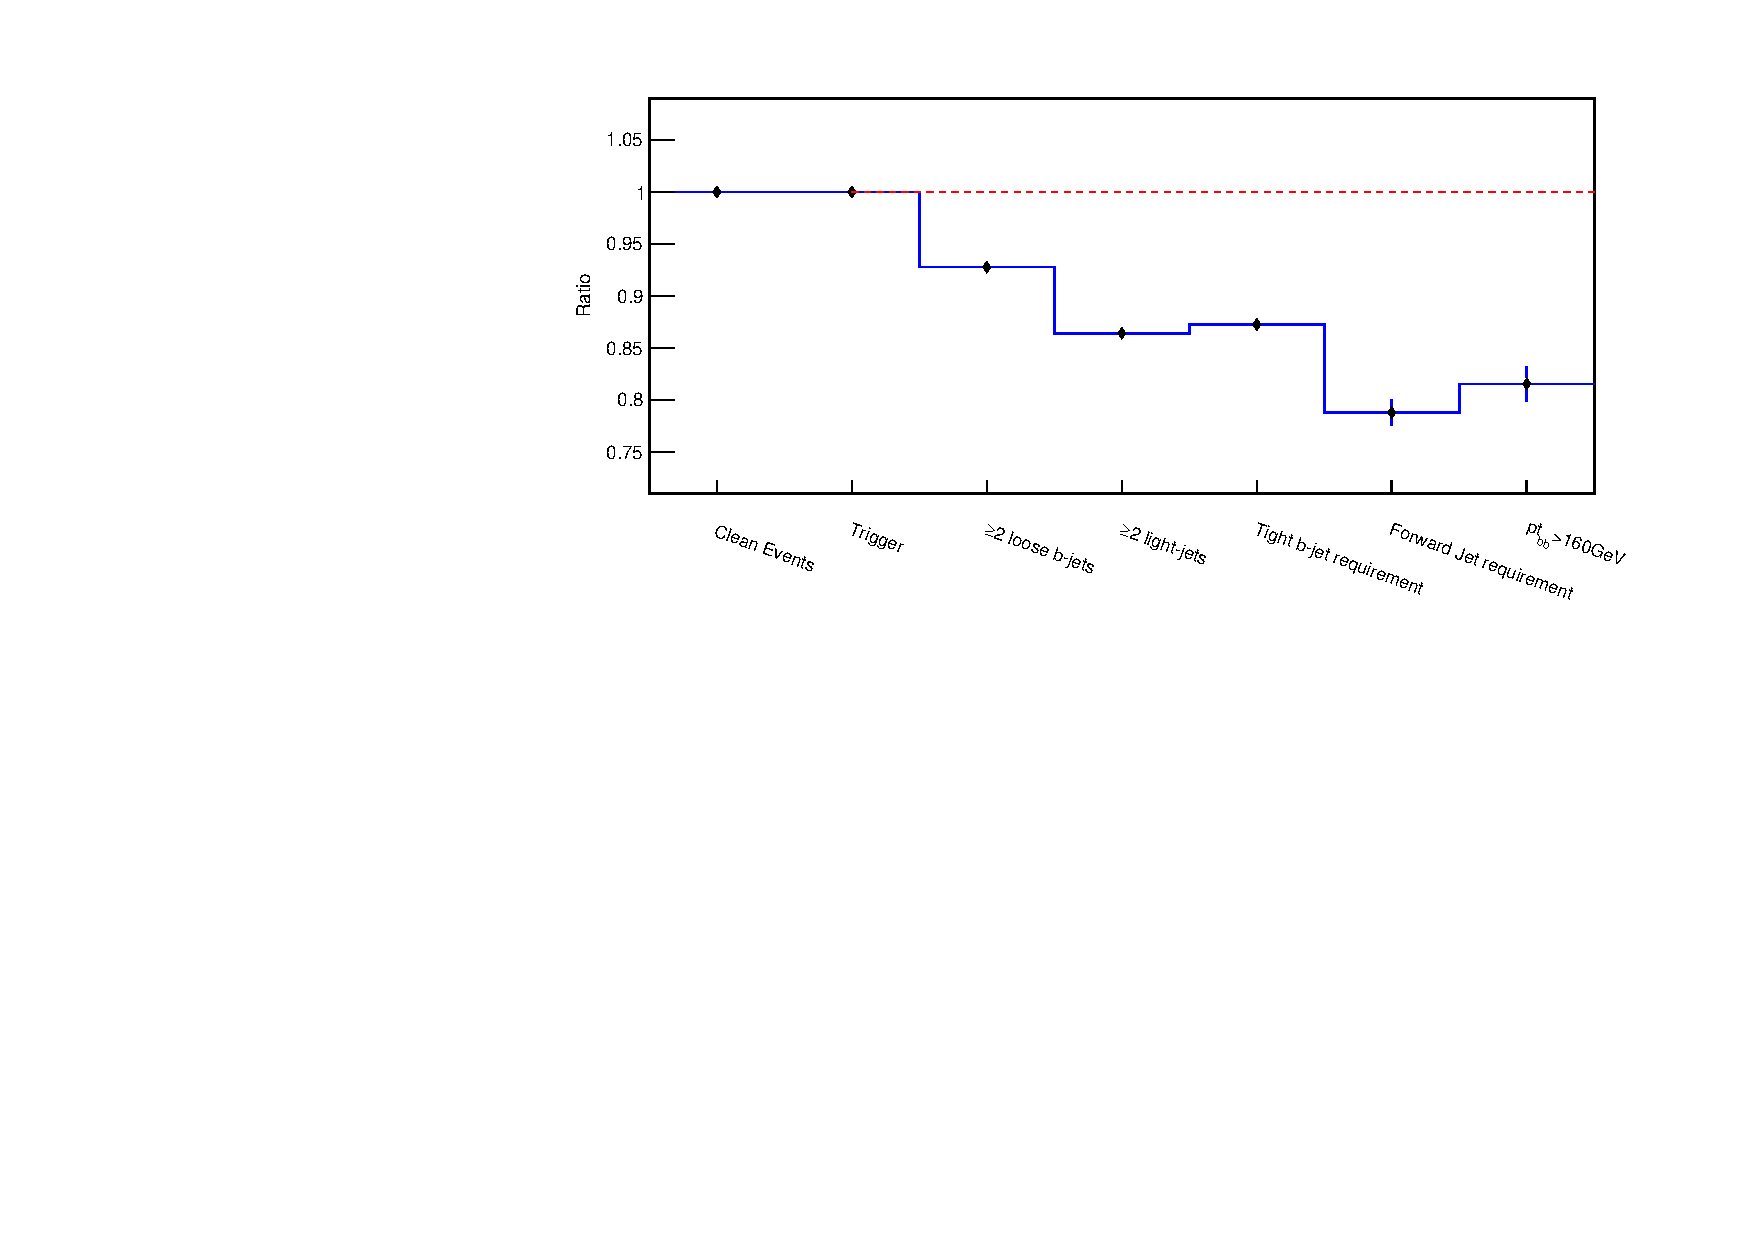
\includegraphics[width=0.75\linewidth]{MC_cutflow}
			\caption{Ratio of the online event count over the offline event count for the Monte-Carlo}
			\label{f:cutflowD}
		\end{figure}

	Overall, the online performance has fewer events than the offline for all points in the cutflow, and overall produces $\sim80\%$ of the total signal events. There are three distinct jumps in the cutflow ratio, at the cuts on the \textit{loose} \bjets\,, light-jets and the forward jet requirement, of $\sim7\%$ each. As shown in Figure \ref{fig:MC:bjetefficiency}, online \btag\, is $\sim93\%$ as efficient as the offline \btag. When considering tagging two distinct \bjets\,, any difference in efficiency is squared. Given the difference in tagging rates, this would result in $\sim86\%$ tagging efficiency for two \bjets\,, which is lower than shown in the cutflow. As shown for the leading \bjet in Section \ref{OP:leadingb}, the offline jet is typically higher in \pt than the online jets. However the difference is small , $\sim2\%$, so any effect on the cutflow should not be as pronounced.

	The $\sim7\%$ drop on the light jet requirement is unexpected, the requirement was solely for 2 jets with \pt$>20$GeV. Given the points above with respect to the \pt difference between online and offline, this drop should not be so sever. The fact the \pt cuts on the light jets were so low also suggests an anomalous result here as such a cut should not contribute a significant reduction in either online or offline.

	Following the drop for the light-jet cut, there is an unexpected increase in the online ratio following the \textit{tight} \btagging\, cut. As highlighted, the tagging efficiency was worse for online than offline, so any requirement for a tagged \bjet\, would be expected to produce a decrease in the online event count relative to the offline count. Perhaps spuriously, the cutflow at this point corresponds to the $86\%$ figure expected given the relative tagging efficiency for two \bjets.

	The final drop occurs following the requirement for a high \pt forward jet. Figure \ref{fig:O:leadingnonbptslice} shows that for non \bjets\, in the forward region of the detector, the \pt of the offline jet is consistently higher than the online \pt. This difference would result in a drop in the online events, with fewer jets passing the threshold \pt cut compared to the offline events.

	Overall for the Monte-Carlo events, there was a 20\% reduction in the number of events that passed the \VBFHBB\, cuts.










	\subsection{Data}
		\begin{figure}[h]
			\centering
			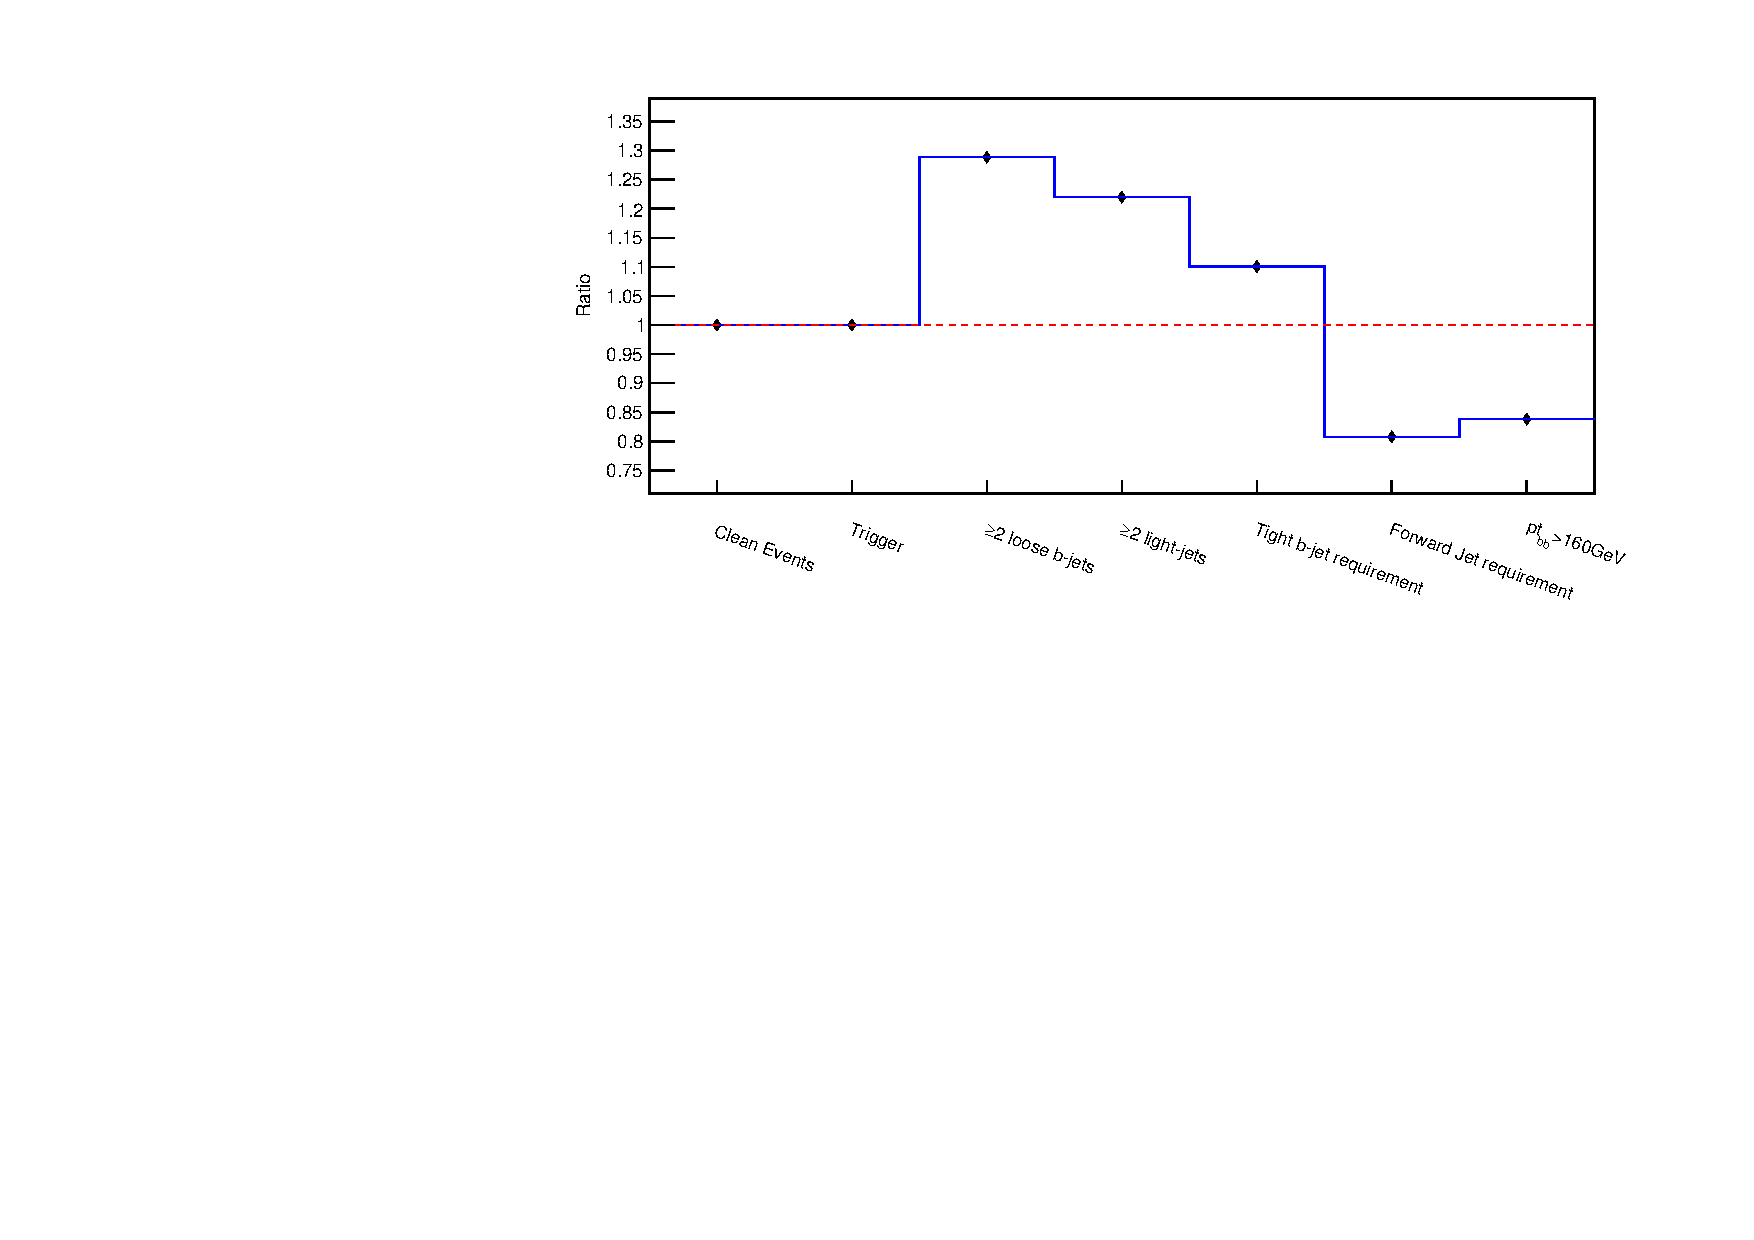
\includegraphics[width=0.75\linewidth]{D_cutflow}
			\caption{Ratio of the online event count over the offline event count for the real data}
			\label{f:cutflowMC}
		\end{figure}




\section{Specific Jet Feature Distributions}

	As the previous chapter showed both \bjets\, and non \bjets\, to be similar for online and offline objects, the kinematic properties of the jets that compose the \VBFHBB\, event are shown to behave similarly.

		\subsubsection{\pt}

			\begin{figure}[h]
				\centering

				\begin{minipage}[h]{0.33\linewidth}
					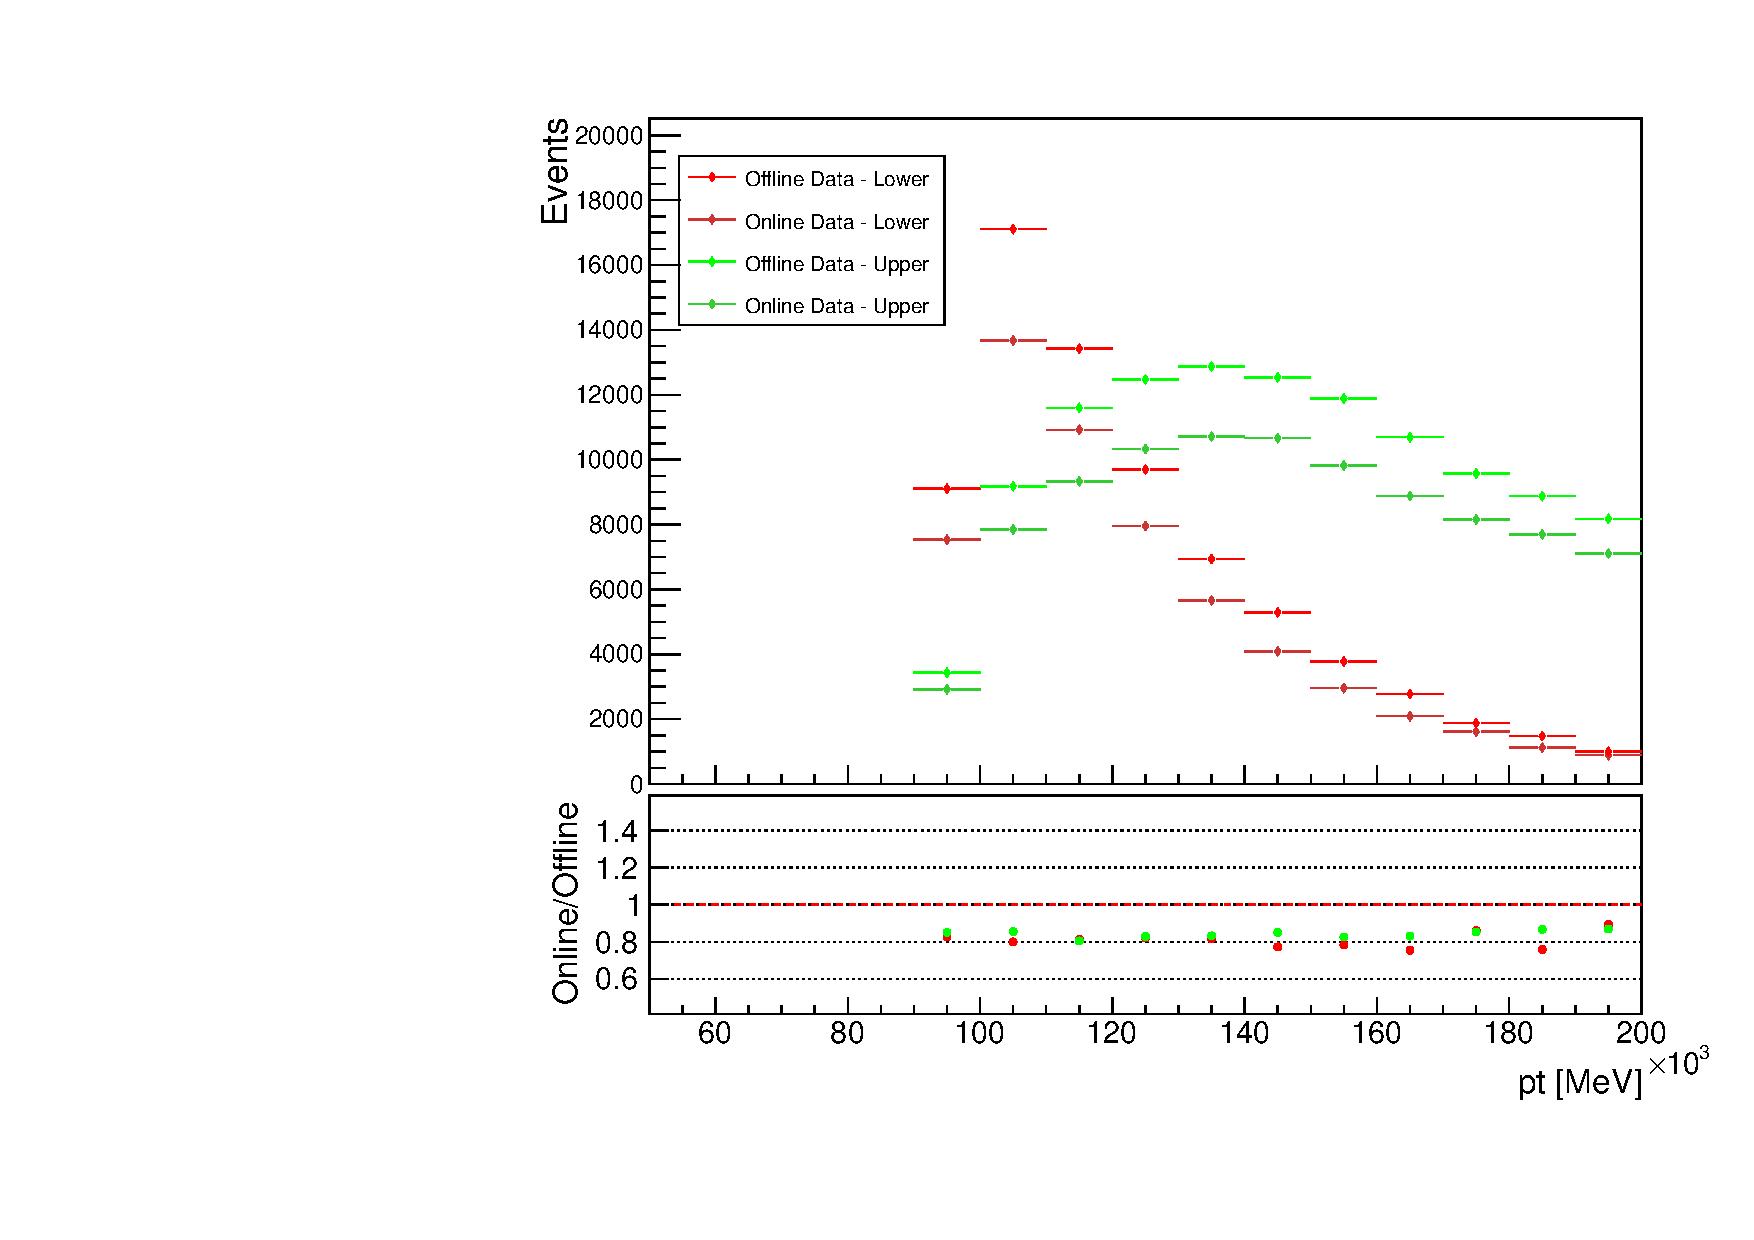
\includegraphics[width=1\linewidth]{pt_bJet1_data_}
				\end{minipage}
				\quad
				\begin{minipage}[h]{0.33\linewidth}
					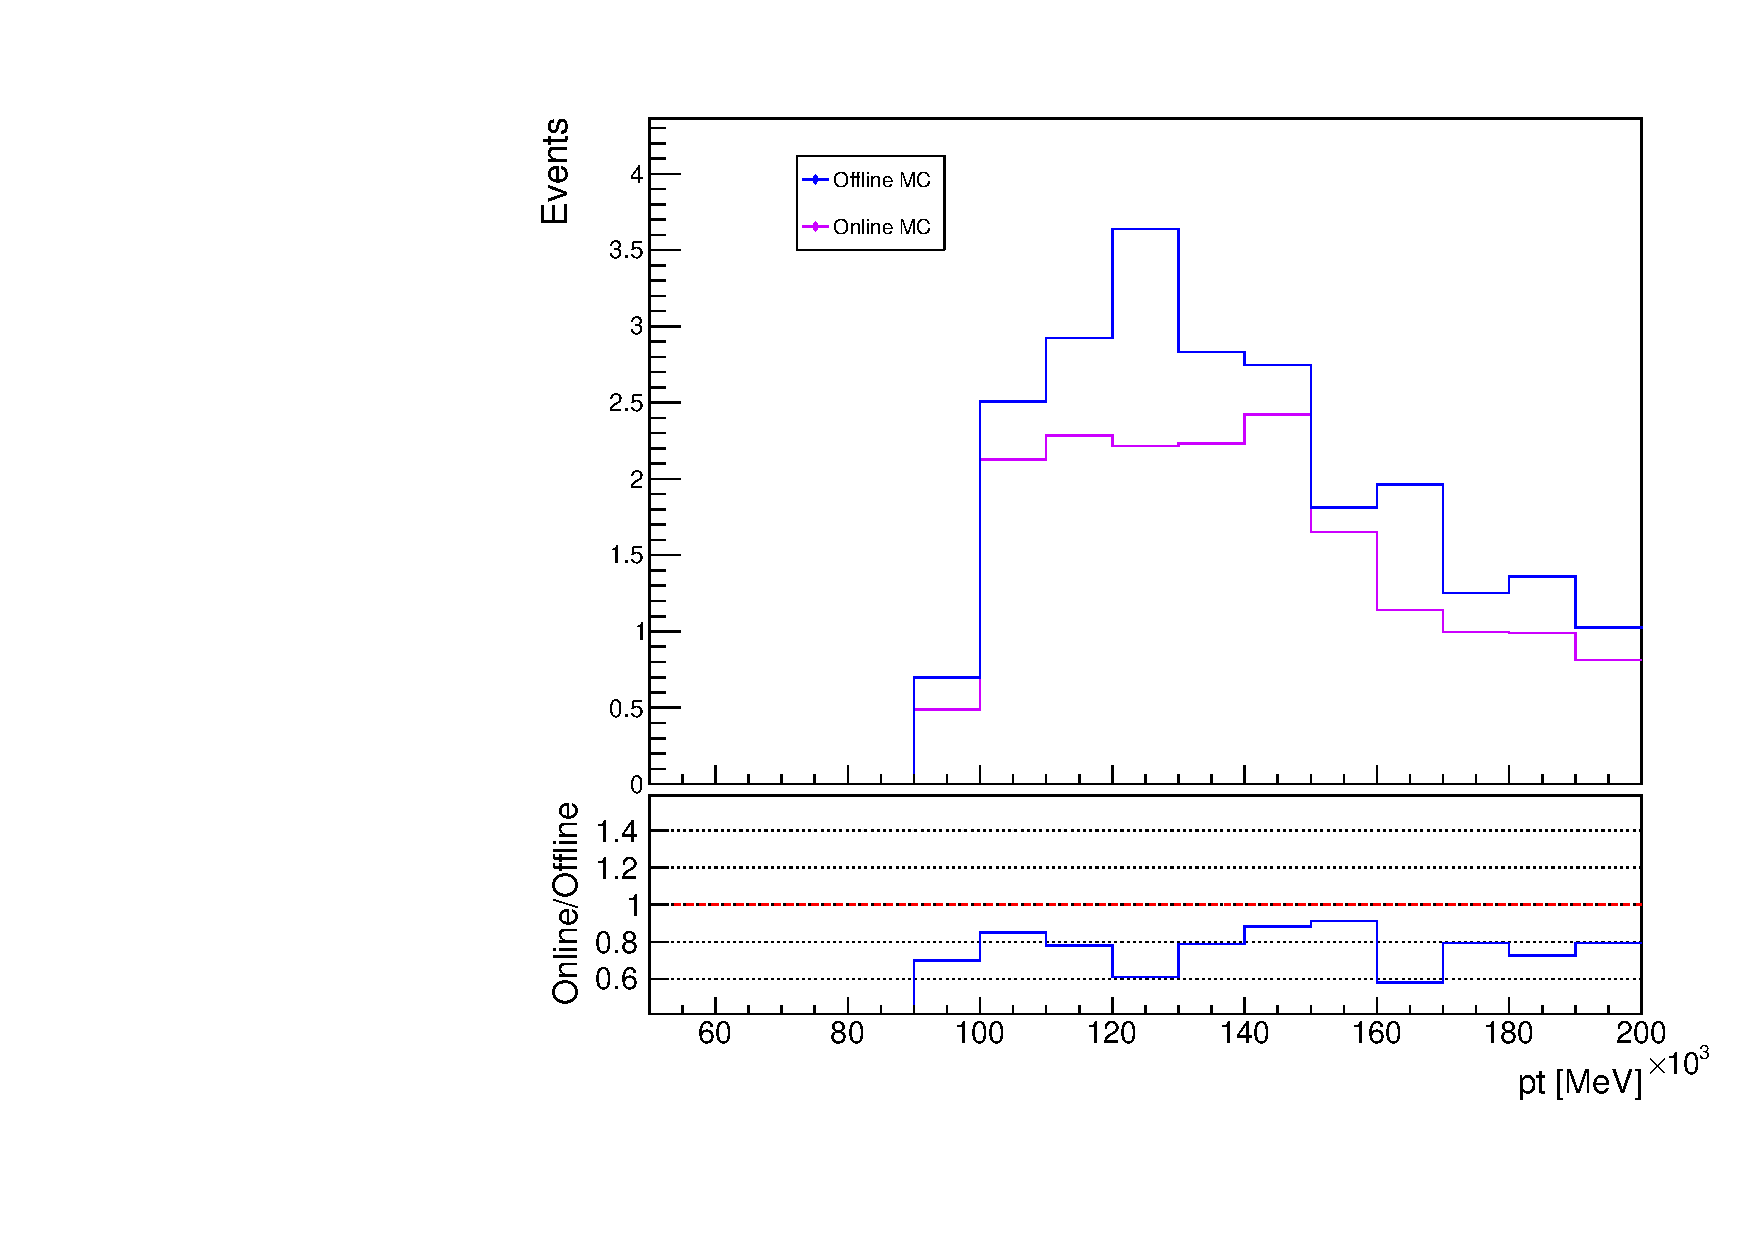
\includegraphics[width=1\linewidth]{pt_bJet1_mc_}
				\end{minipage}

				\begin{minipage}[h]{0.33\linewidth}
					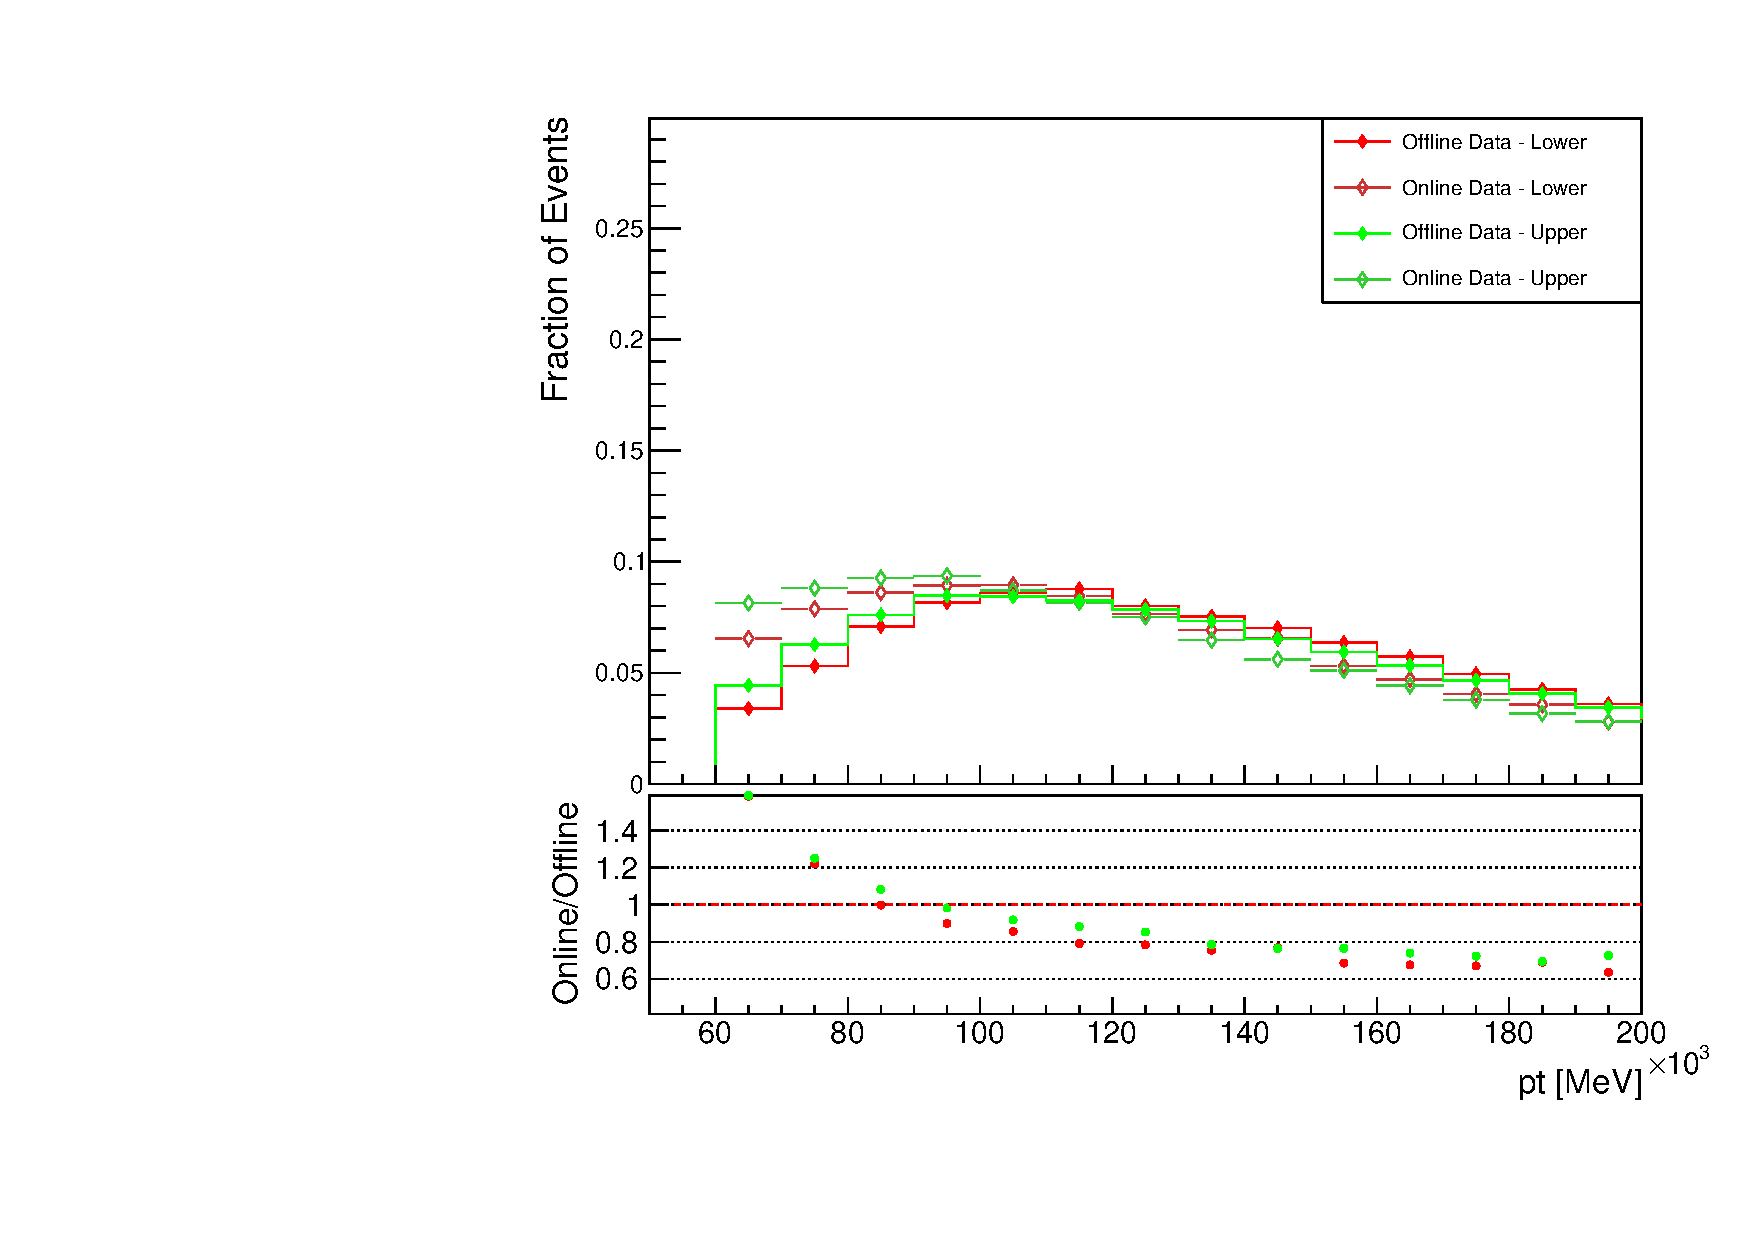
\includegraphics[width=1\linewidth]{pt_lJet1_data_}
				\end{minipage}
				\quad
				\begin{minipage}[h]{0.33\linewidth}
					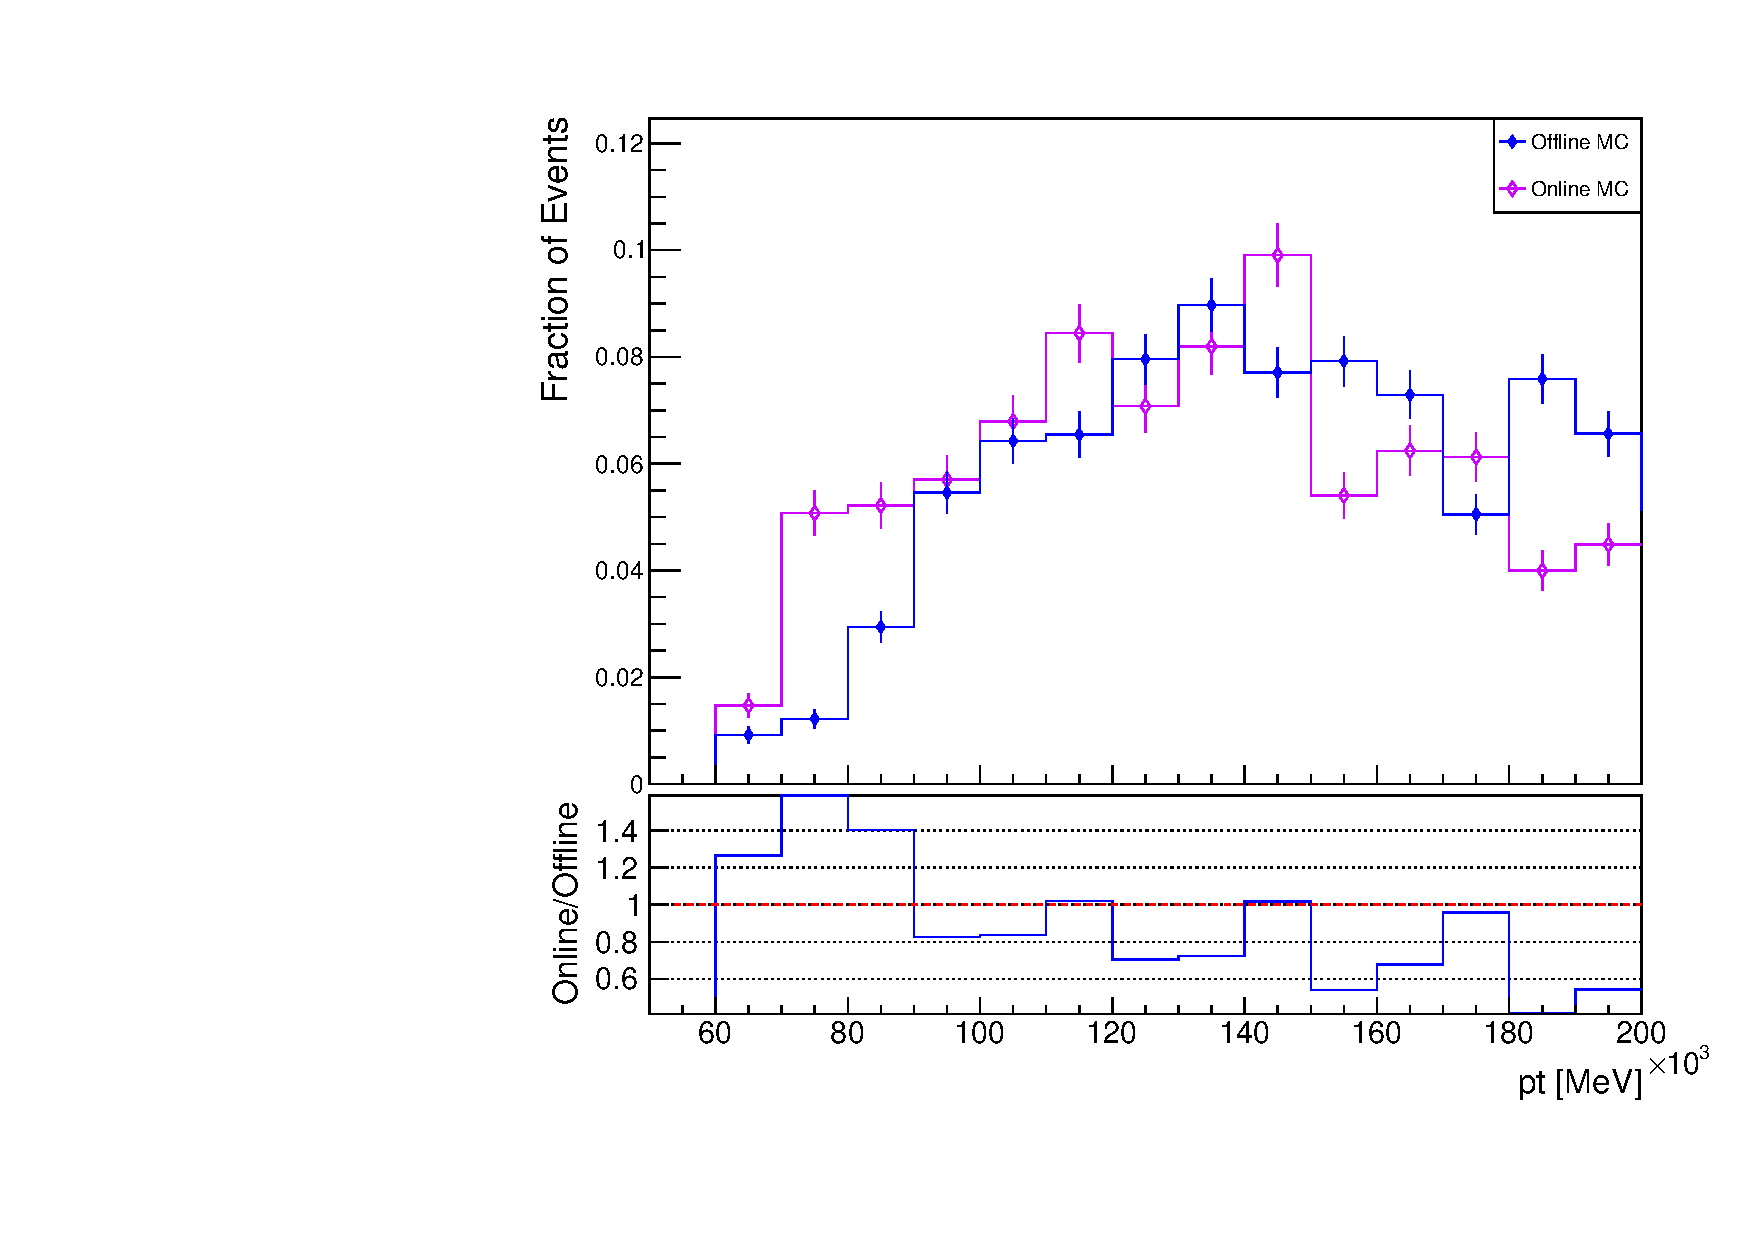
\includegraphics[width=1\linewidth]{pt_lJet1_mc_}
				\end{minipage}

			\end{figure}



			\subsubsection{$\eta$}

				\begin{figure}[h]
					\centering

					\begin{minipage}[h]{0.33\linewidth}
						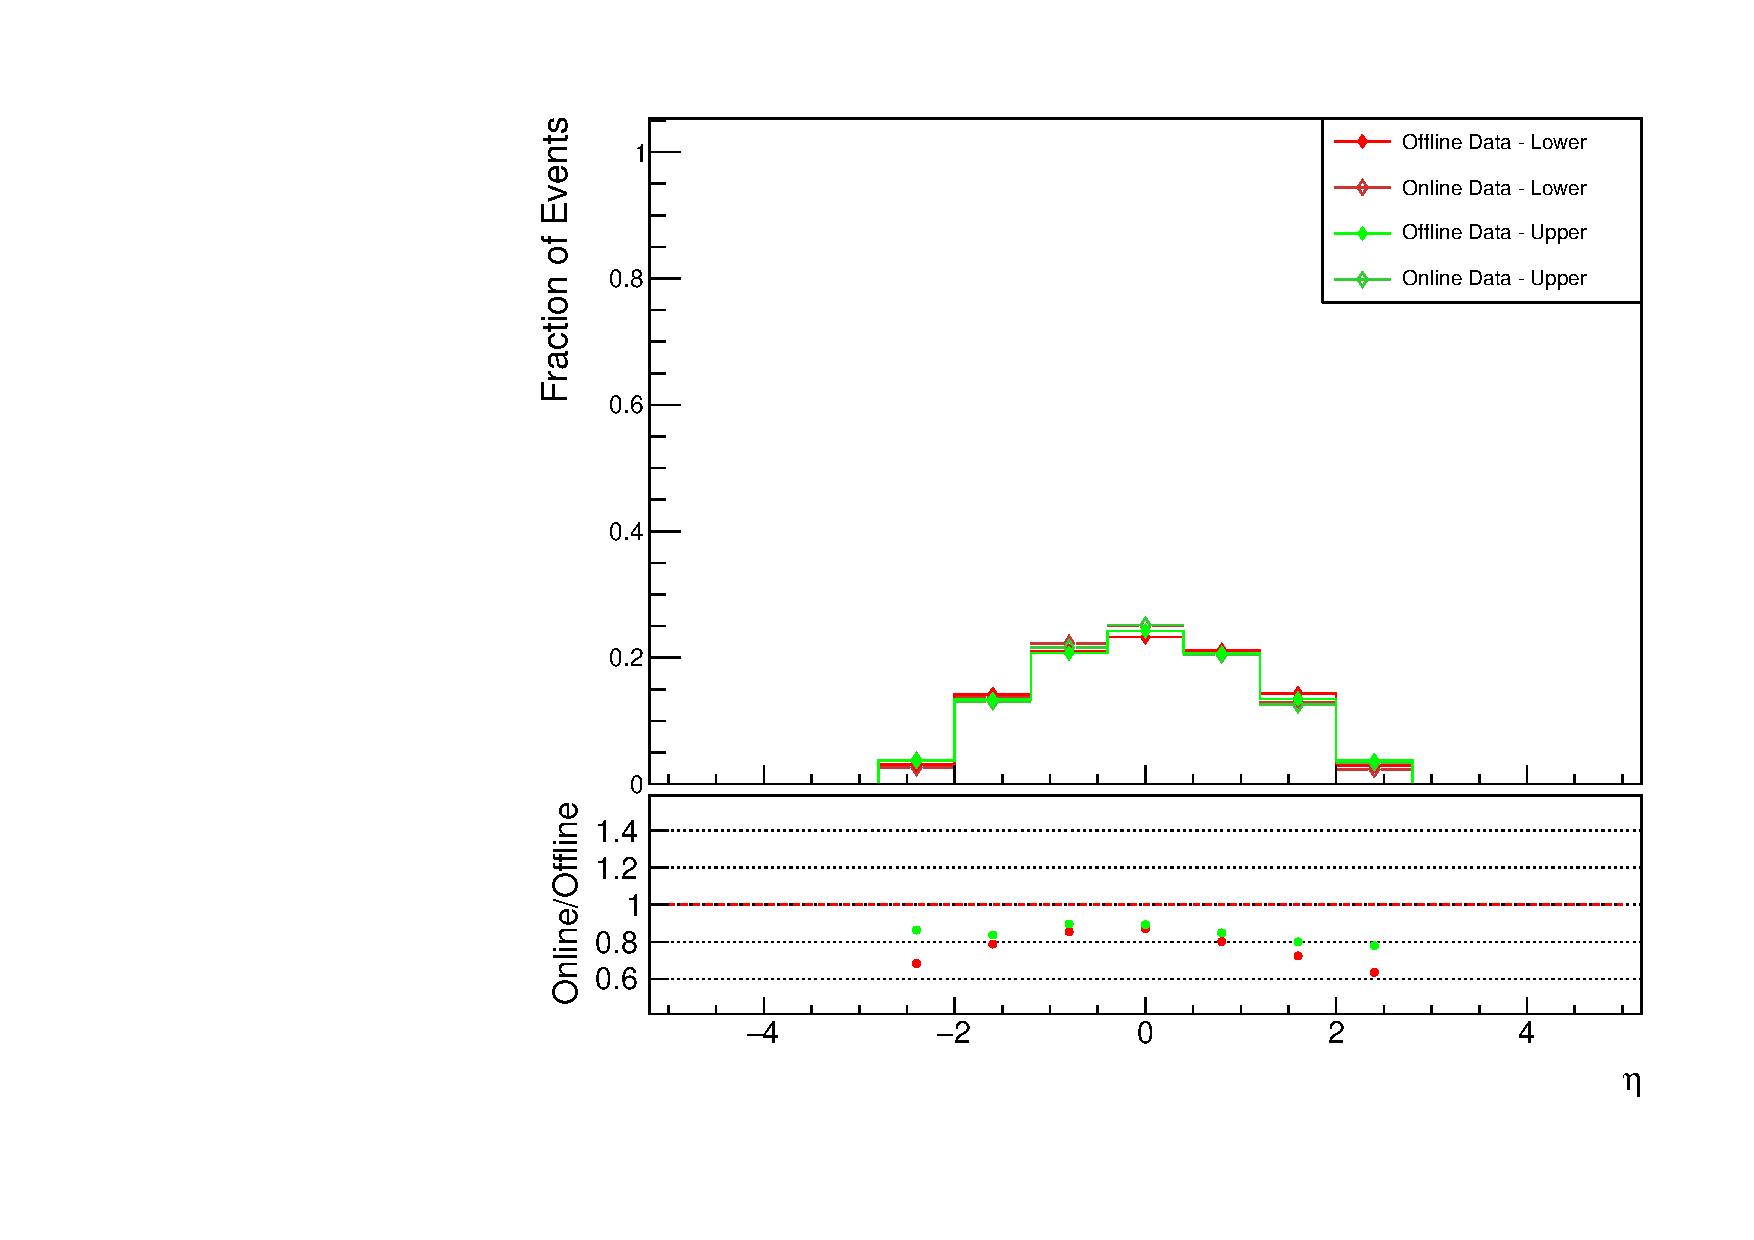
\includegraphics[width=1\linewidth]{eta_bJet1_data_}
					\end{minipage}
					\quad
					\begin{minipage}[h]{0.33\linewidth}
						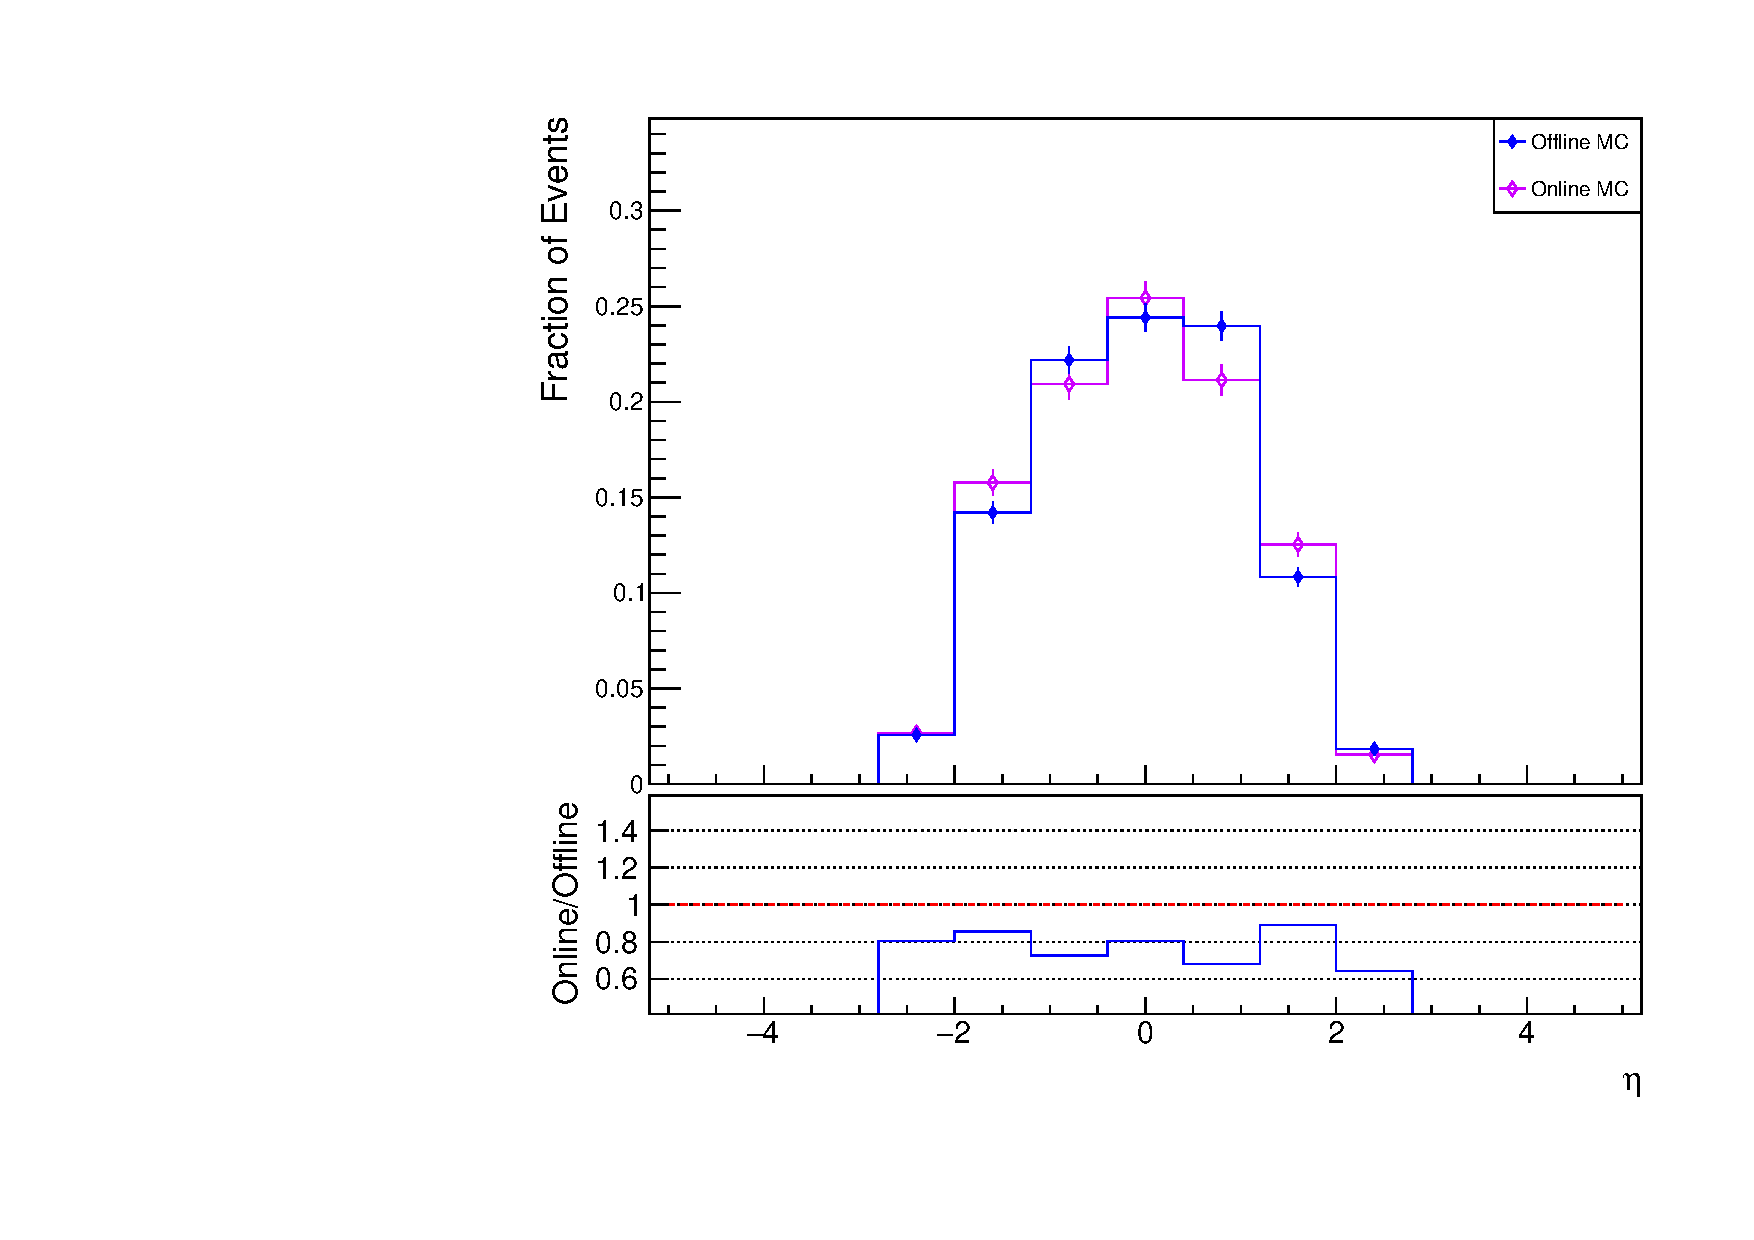
\includegraphics[width=1\linewidth]{eta_bJet1_mc_}
					\end{minipage}

					\begin{minipage}[h]{0.33\linewidth}
						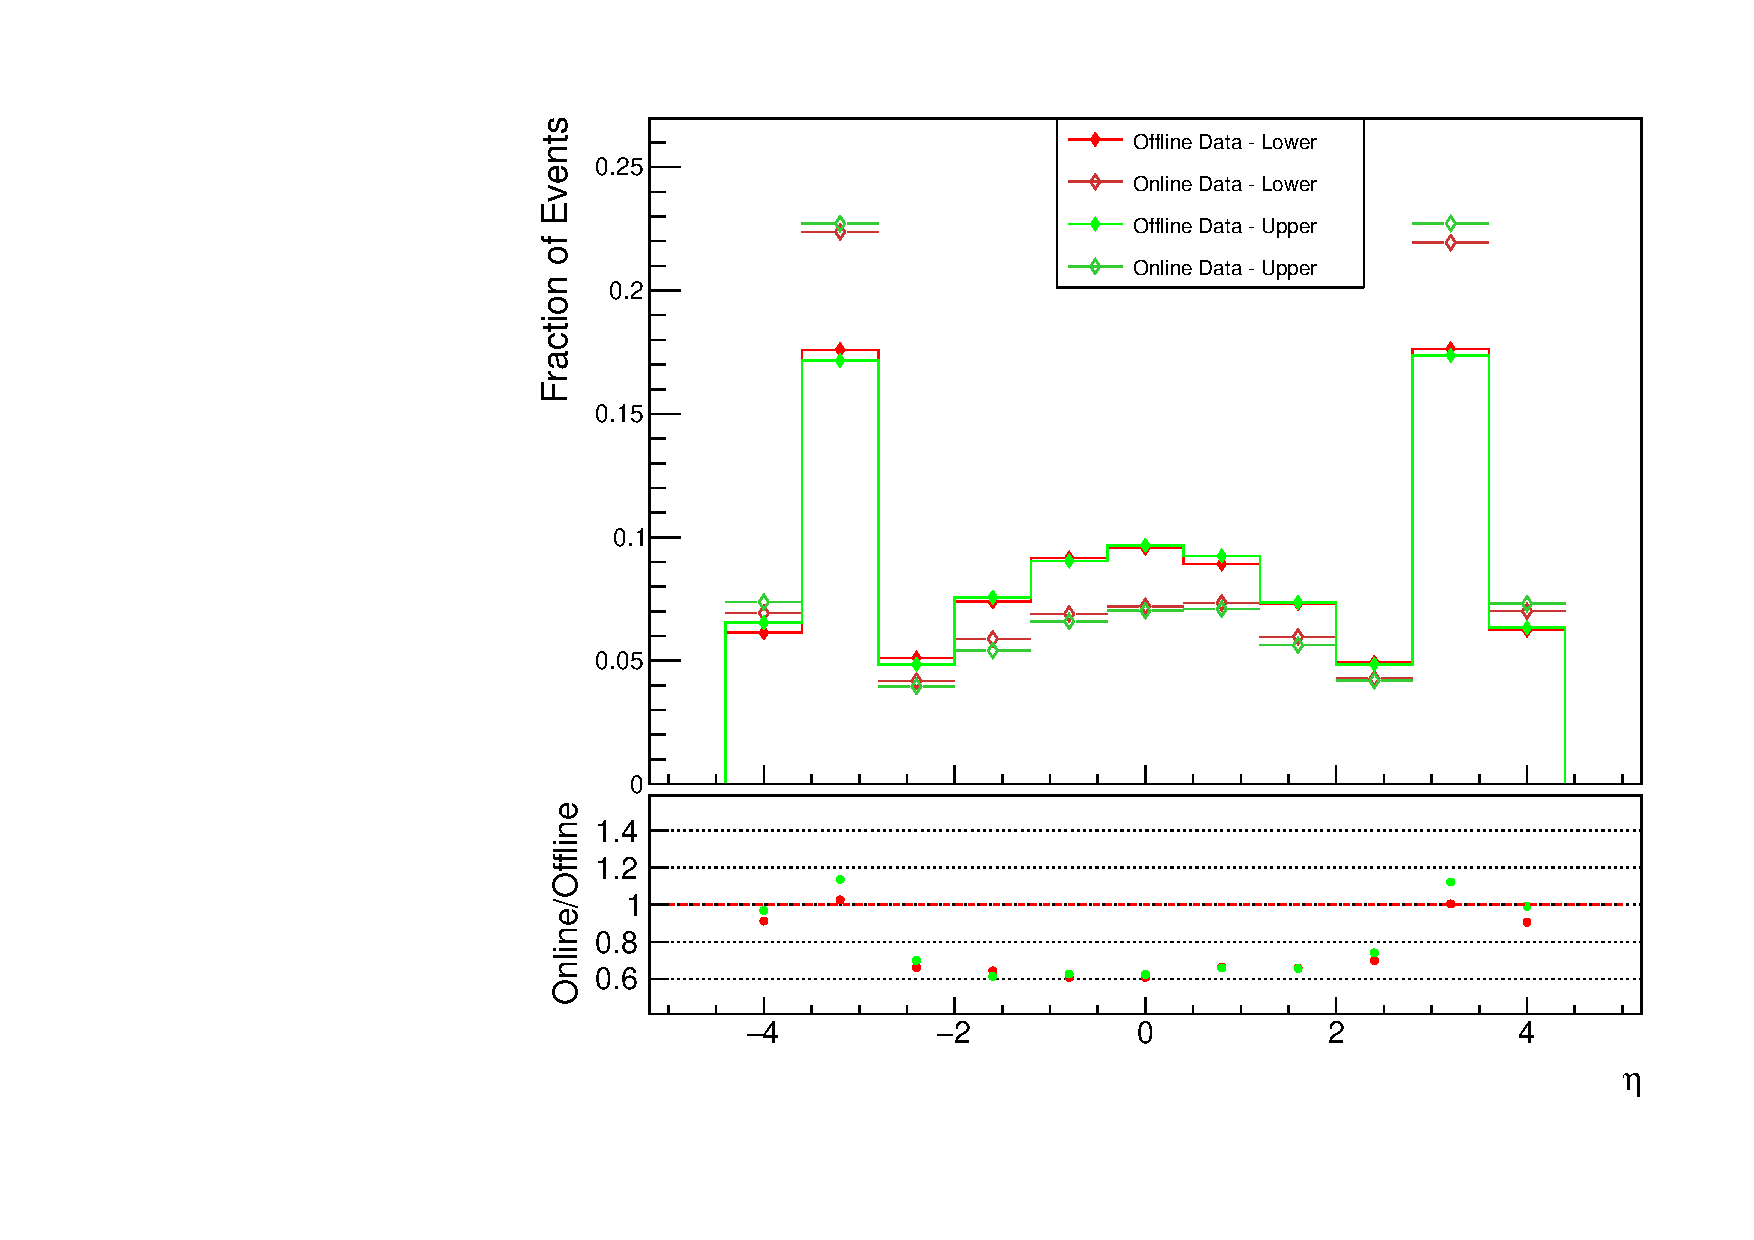
\includegraphics[width=1\linewidth]{eta_lJet1_data_}
					\end{minipage}
					\quad
					\begin{minipage}[h]{0.33\linewidth}
						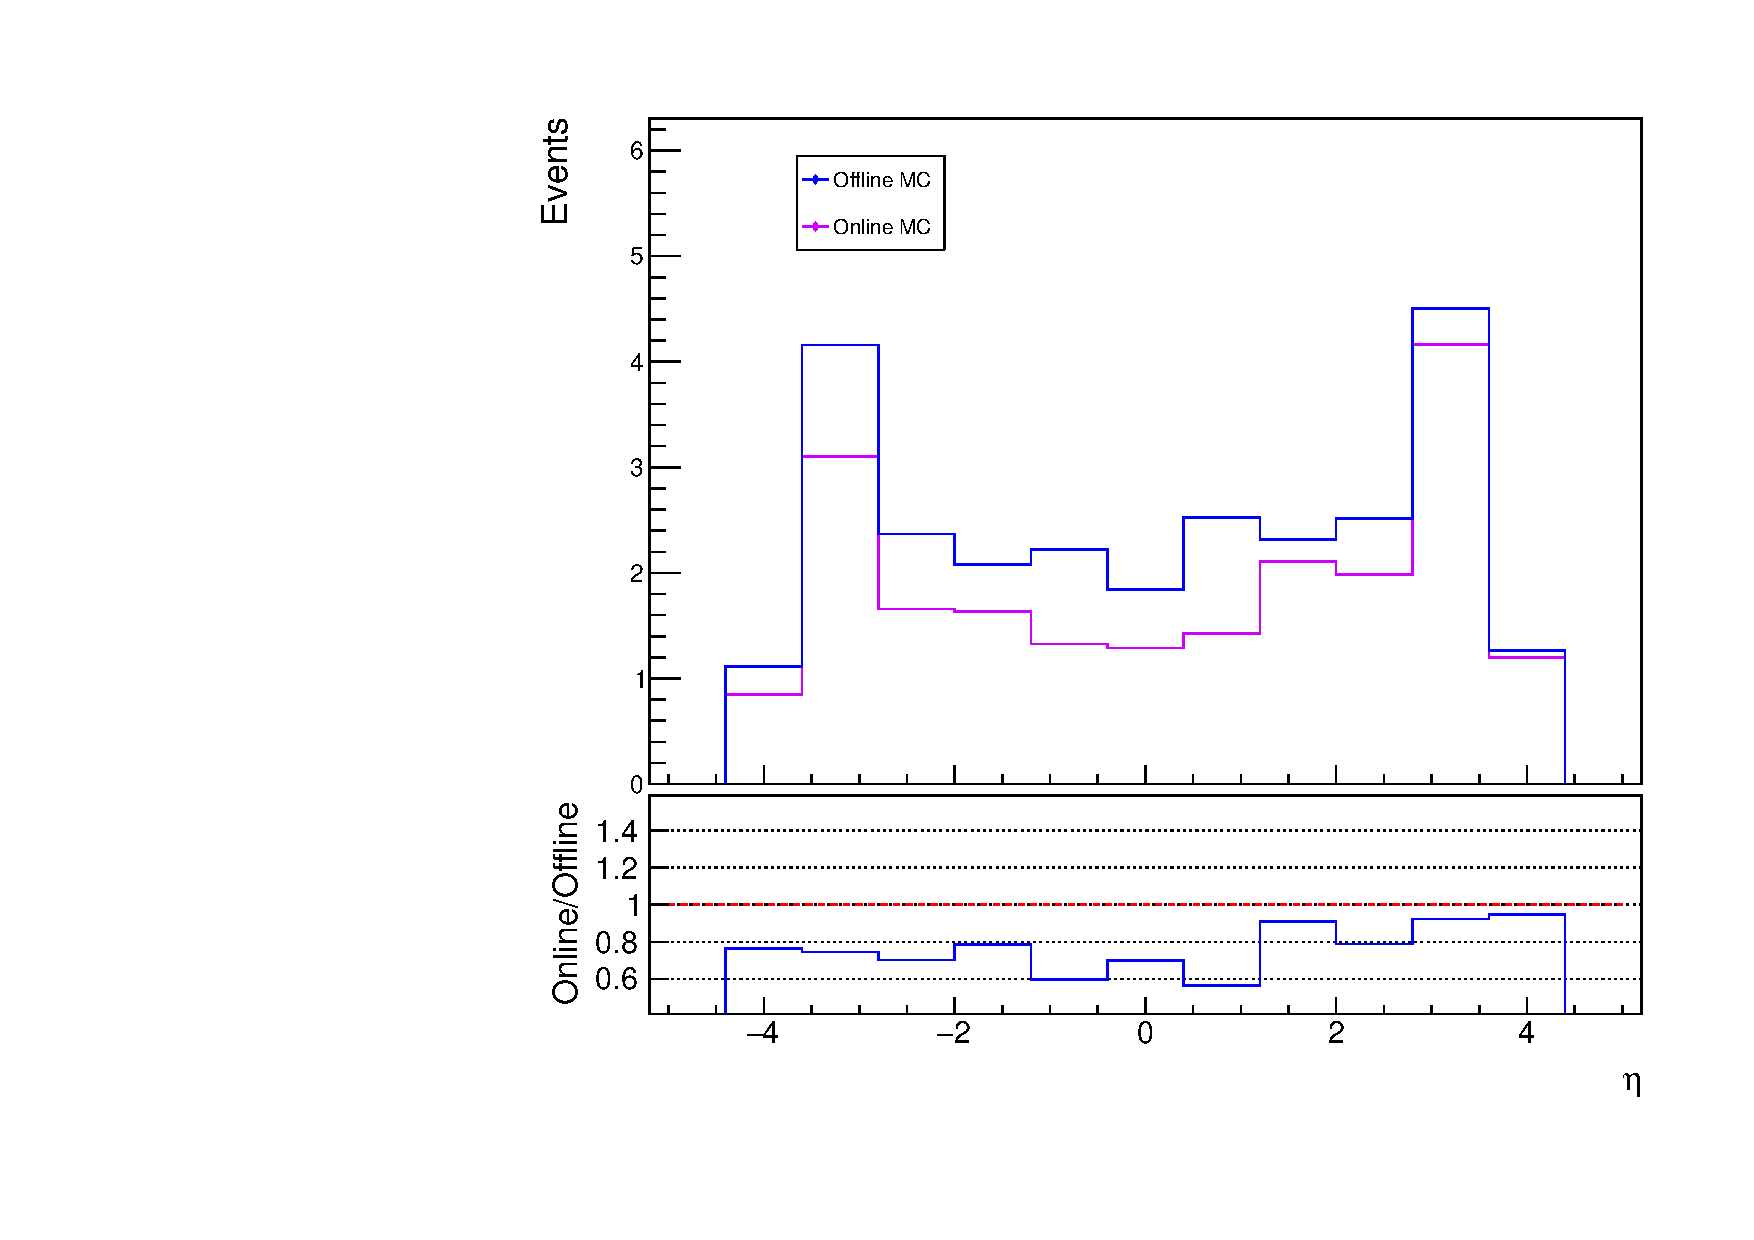
\includegraphics[width=1\linewidth]{eta_lJet1_mc_}
					\end{minipage}
					\label{fig:kin:eta2c4j}
				\end{figure}


\section{BDT Input Variables}

	\begin{itemize}
		\item $M_{jj}$
		\item \pt$_{jj}$
		\item $\cos \theta$
		\item $\Delta\eta_{jj}$
		\item $Max(\eta)$
		\item $\eta*$
		\item $min\Delta R(j_1)$
		\item $min\Delta R(j_1)$
		\item \pt balance
		\item $N_{TRK}(j_1) PV500$ ?
		\item $N_{TRK}(j_) PV500$ ?
	\end{itemize}

		\begin{figure}[h]
			\centering1
			\begin{minipage}[h]{0.45\linewidth}
				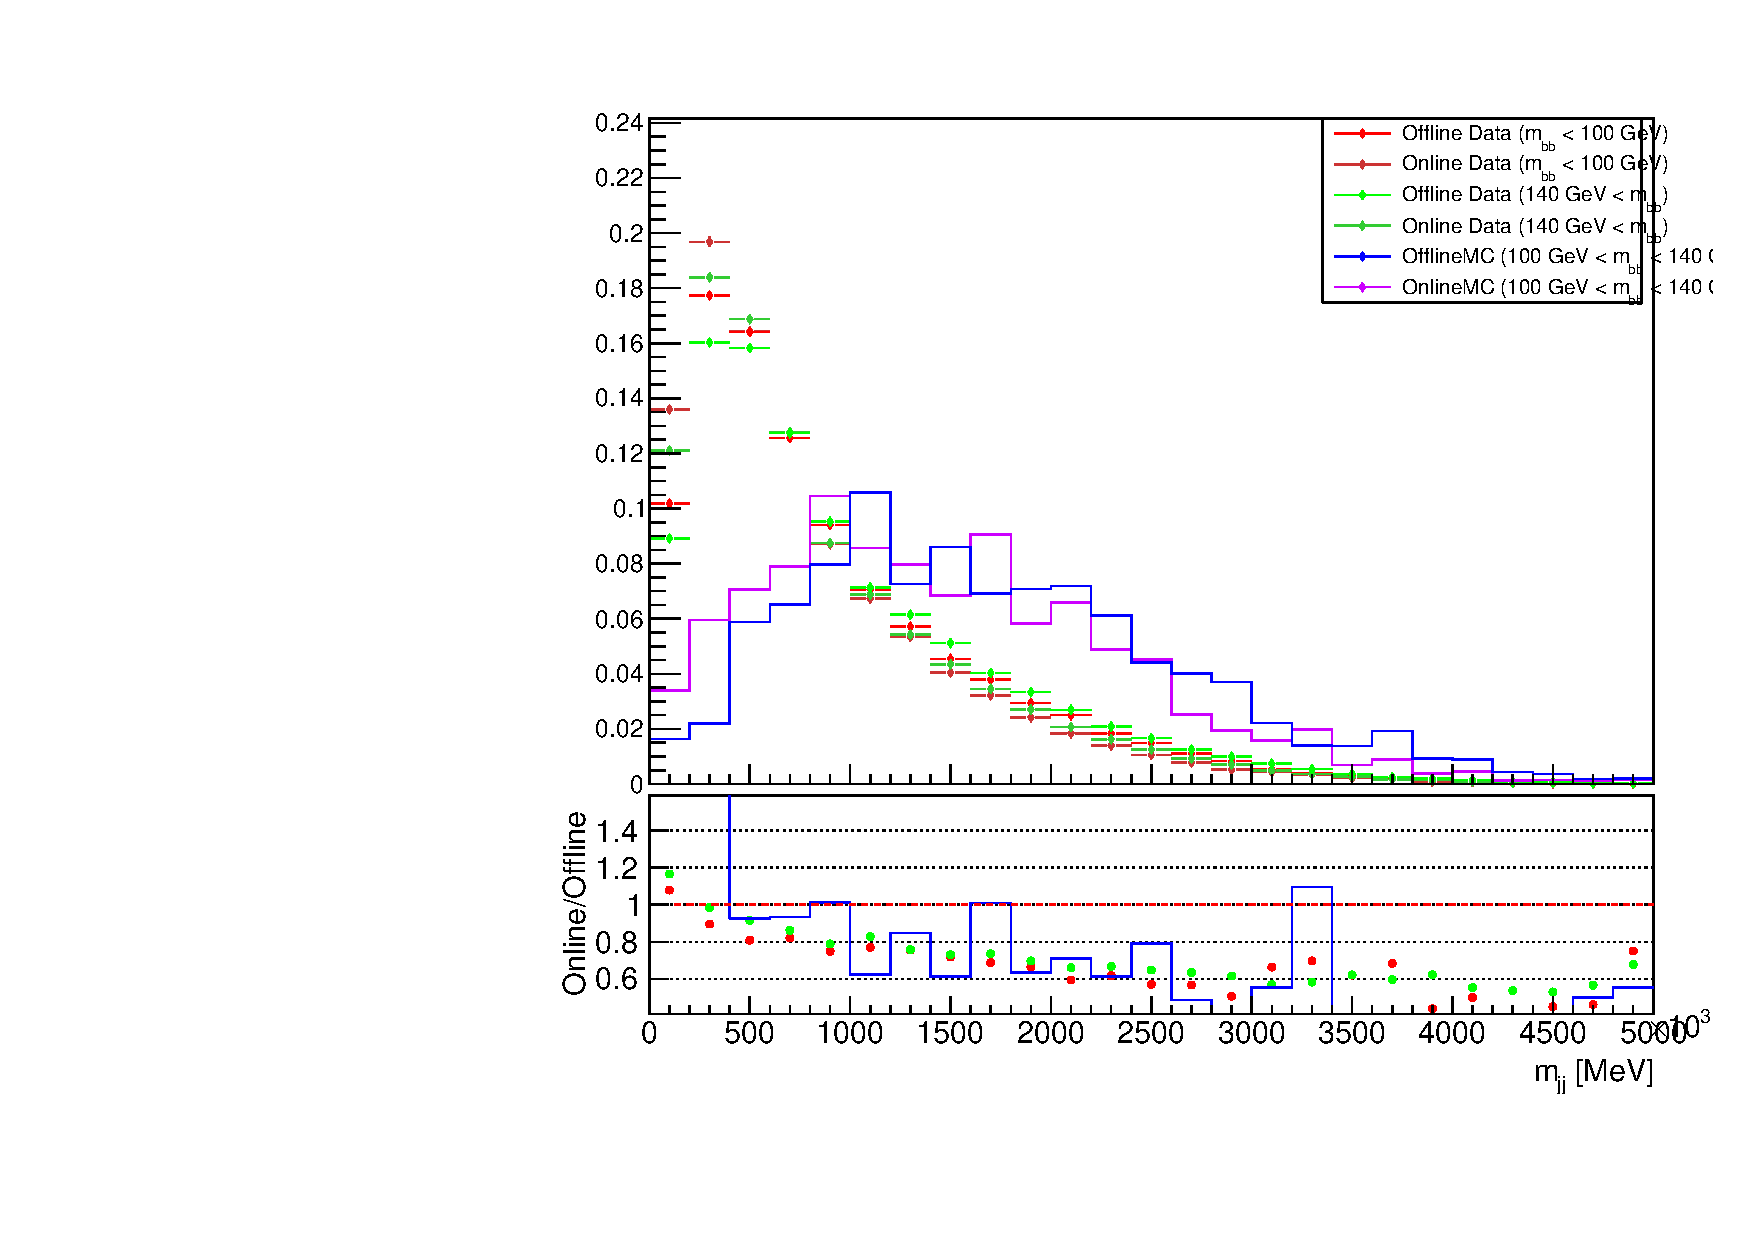
\includegraphics[width=1\linewidth]{mjj}
				\caption{}
				\label{fig:bdtmjj}
			\end{minipage}
			\quad
			\begin{minipage}[h]{0.45\linewidth}
				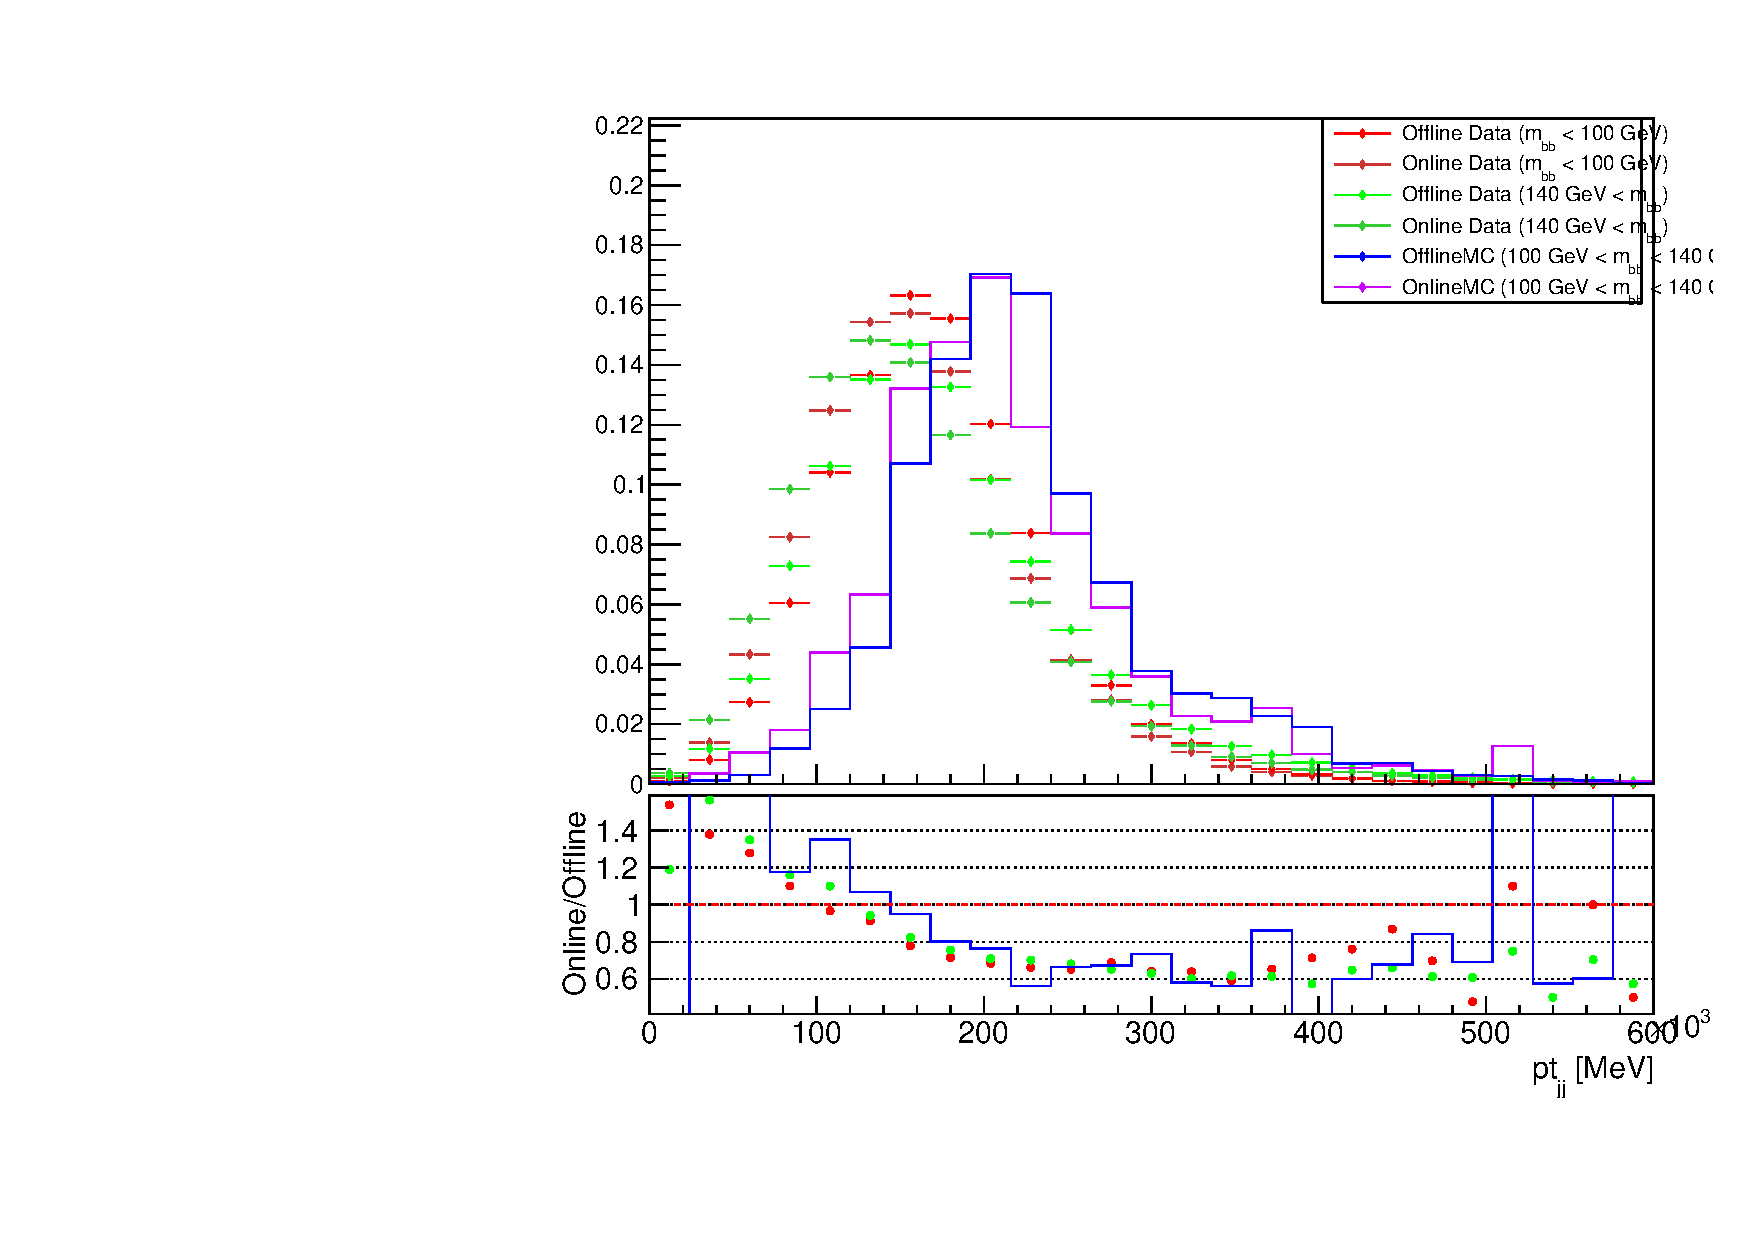
\includegraphics[width=1\linewidth]{ptjj}
				\caption{}
				\label{fig:bdtptjj}
			\end{minipage}
		\end{figure}

		\begin{figure}[h]
			\centering
			\begin{minipage}[h]{0.45\linewidth}
				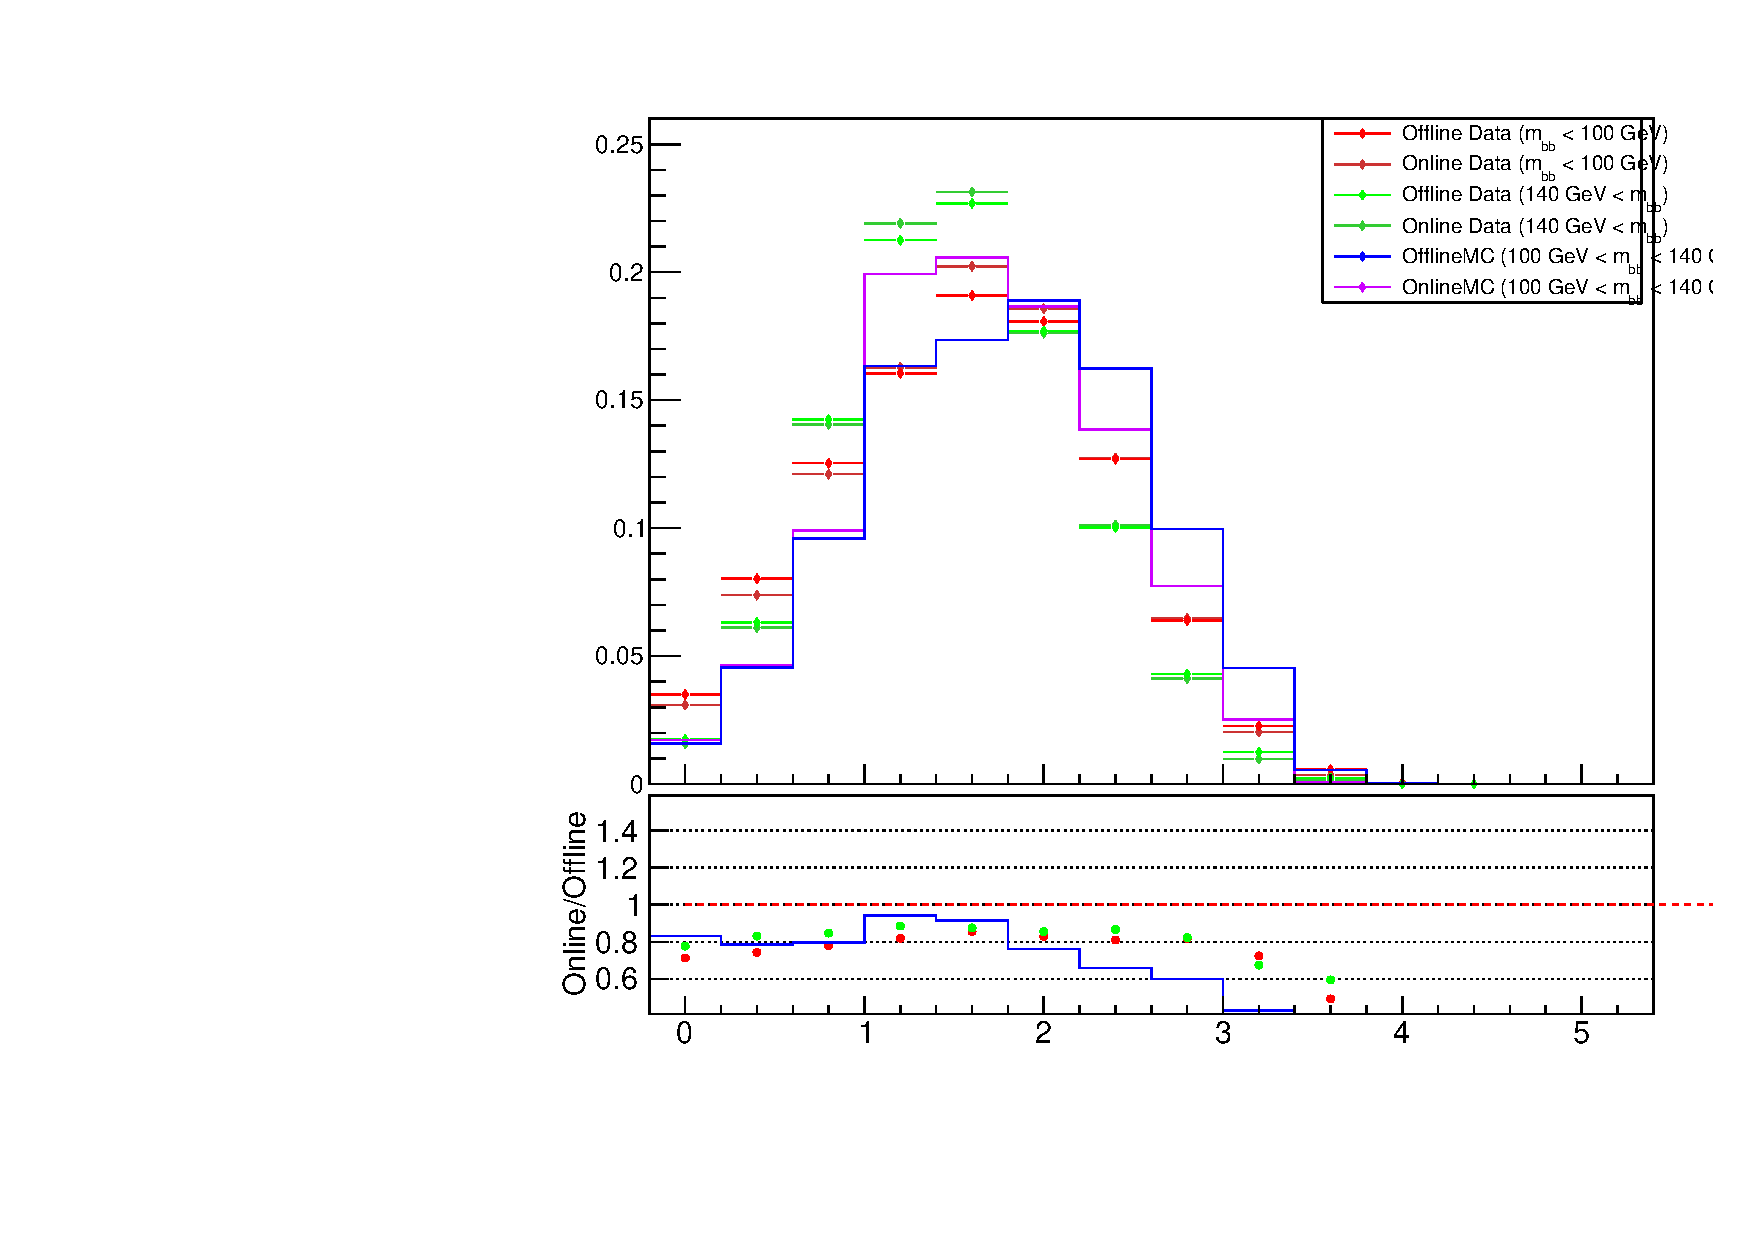
\includegraphics[width=1\linewidth]{etastar}
				\caption{}
				\label{fig:bdtetastar}
			\end{minipage}
			\quad
			\begin{minipage}[h]{0.45\linewidth}
				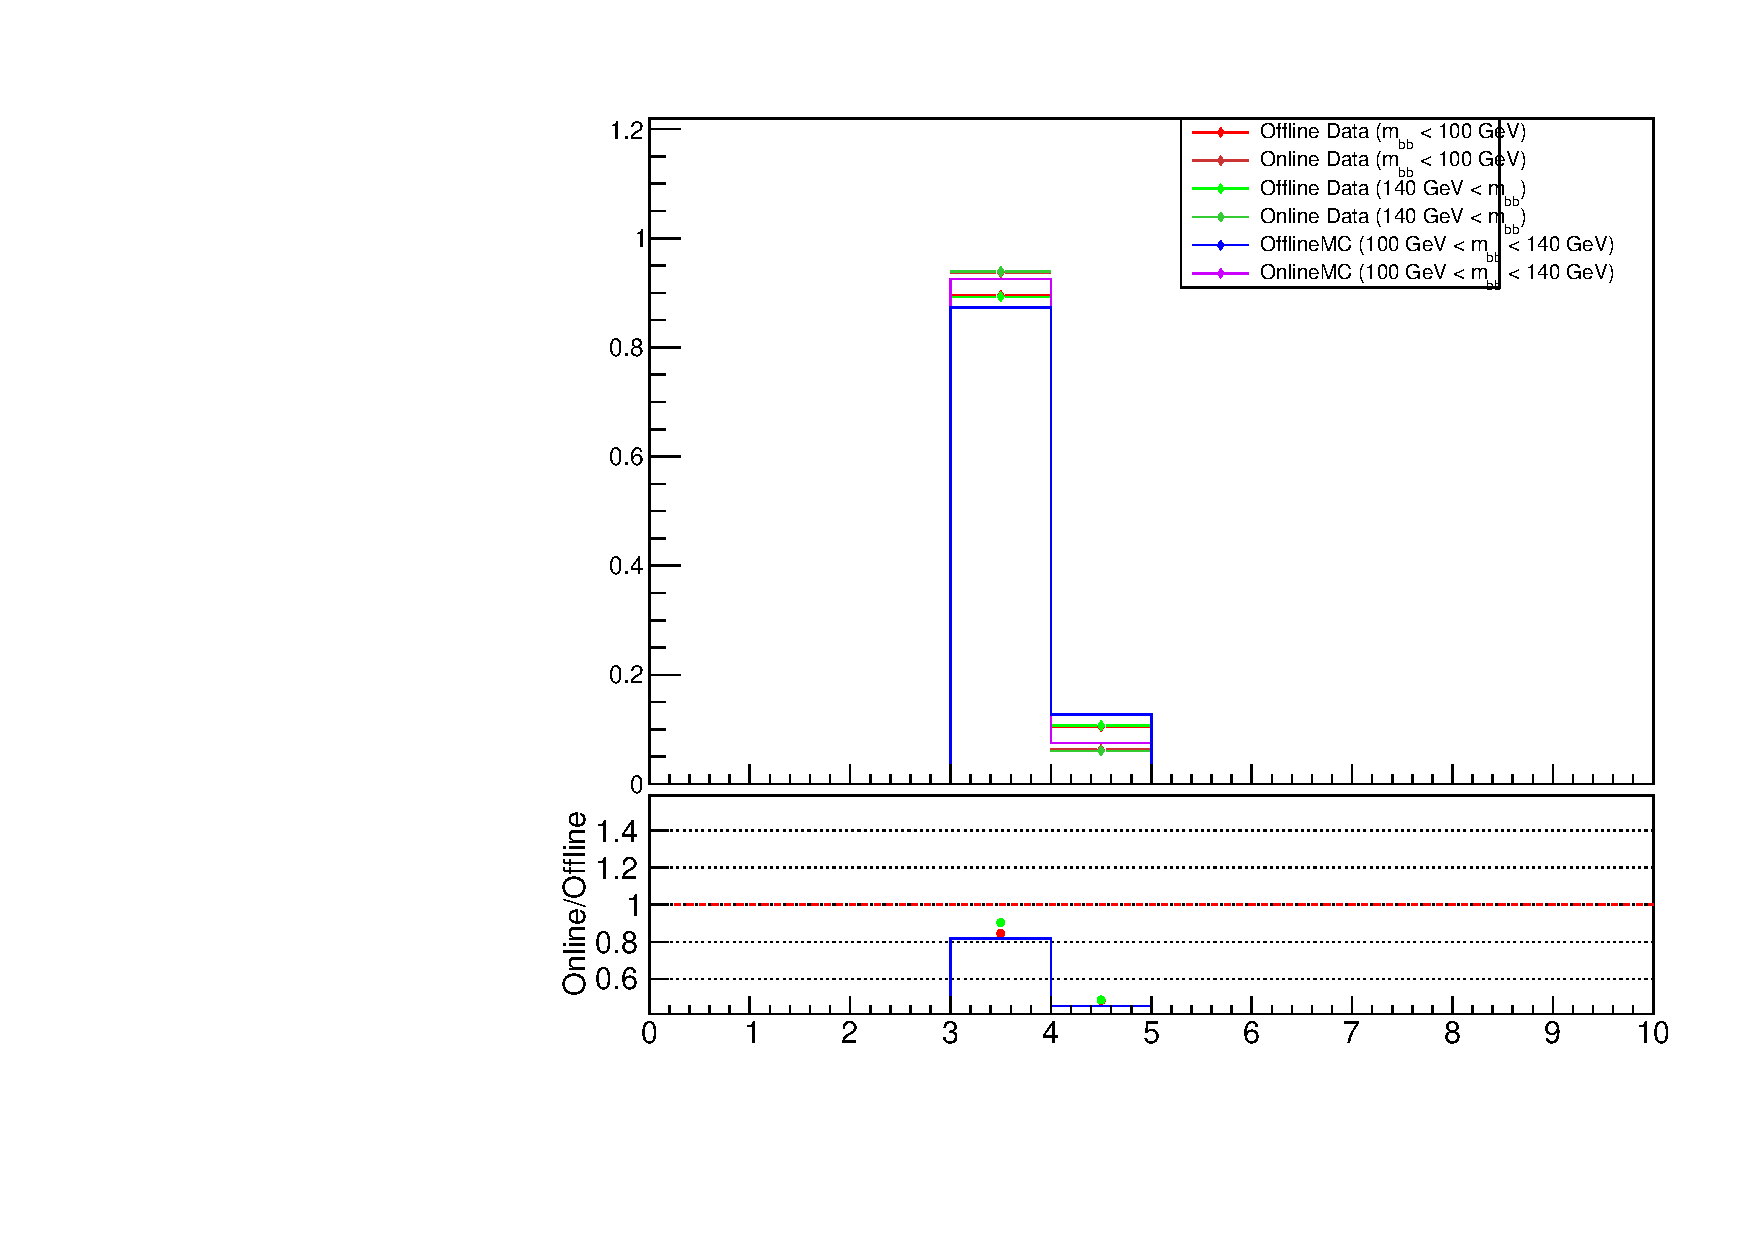
\includegraphics[width=1\linewidth]{maxeta}
				\caption{}
				\label{fig:bdtmaxeta}
			\end{minipage}
		\end{figure}

		\begin{figure}[h]
			\centering
			\begin{minipage}[h]{0.45\linewidth}
				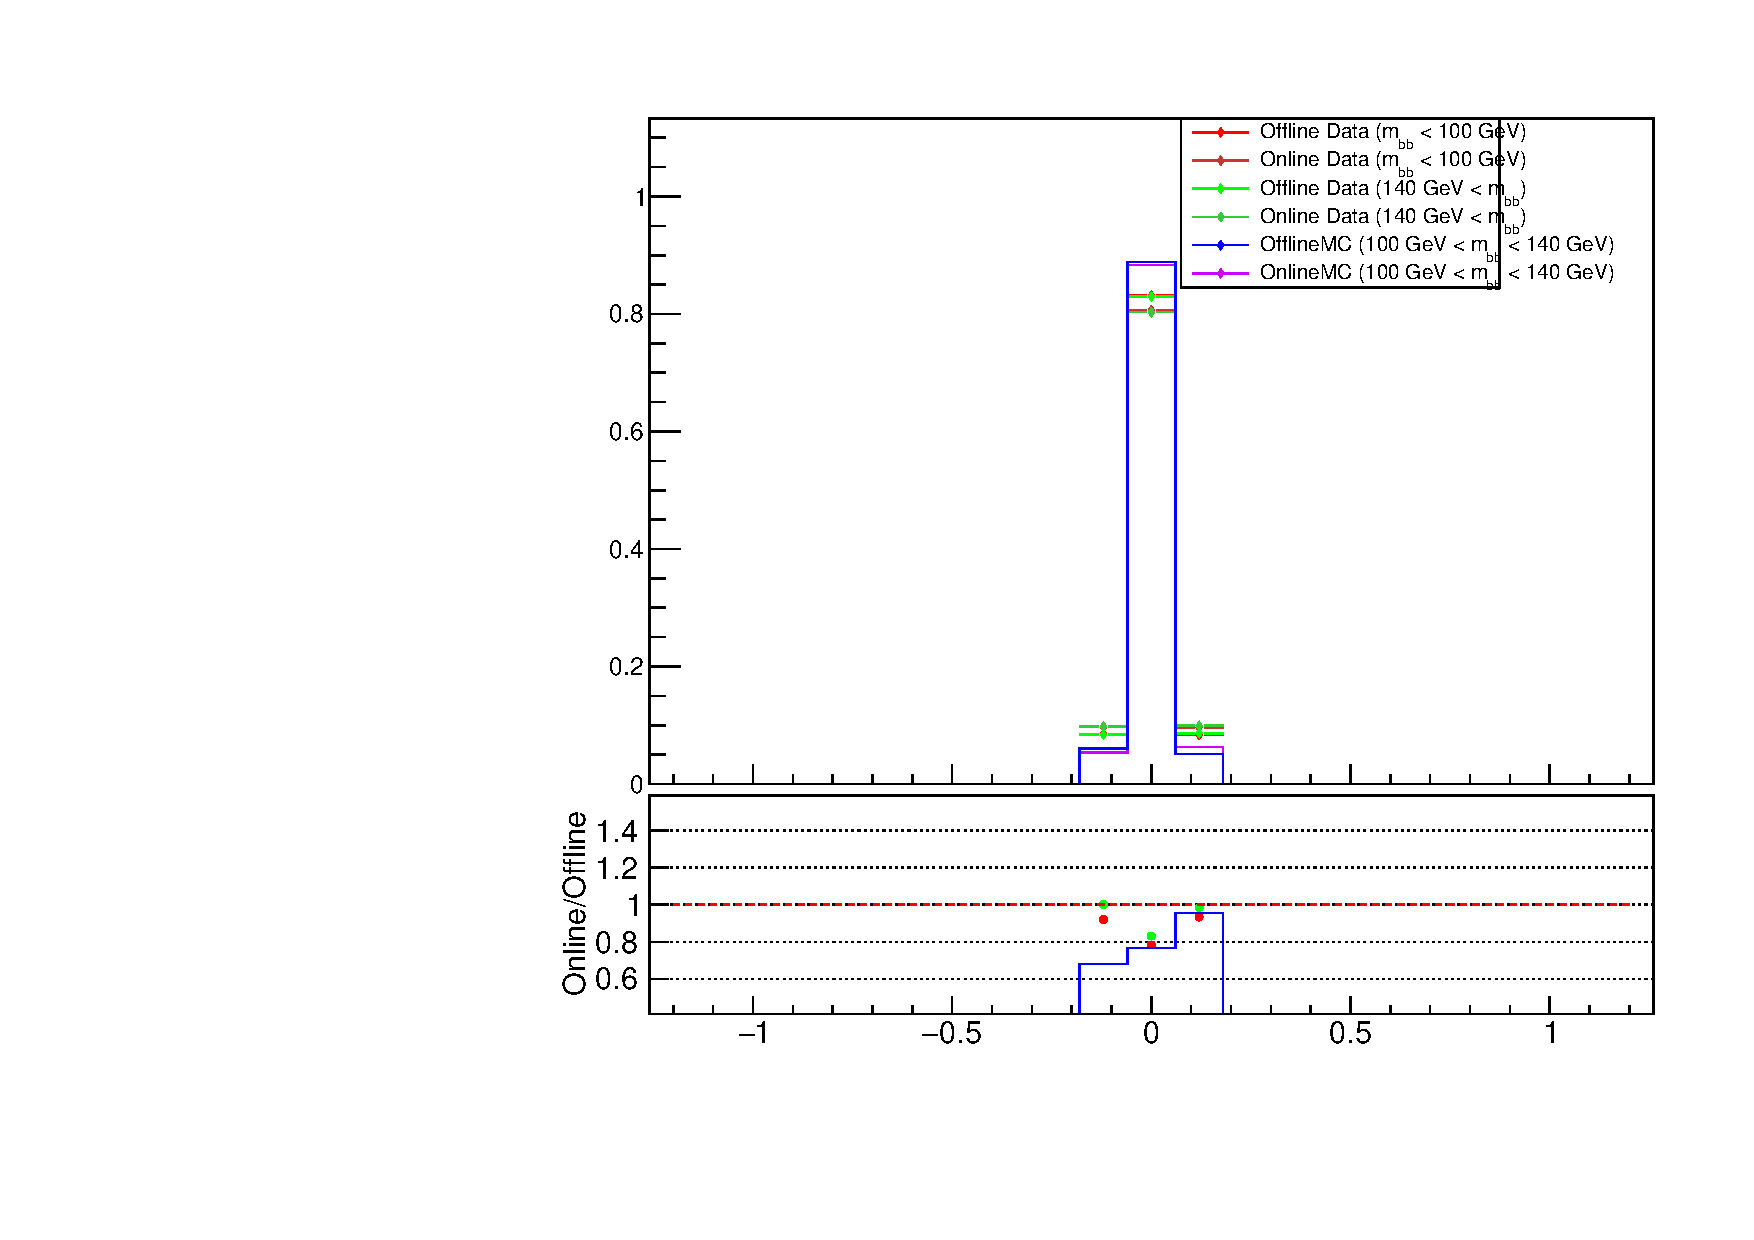
\includegraphics[width=1\linewidth]{costheta}
				\caption{}
				\label{fig:bdtcpostheta}
			\end{minipage}
			\quad
			\begin{minipage}[h]{0.45\linewidth}
				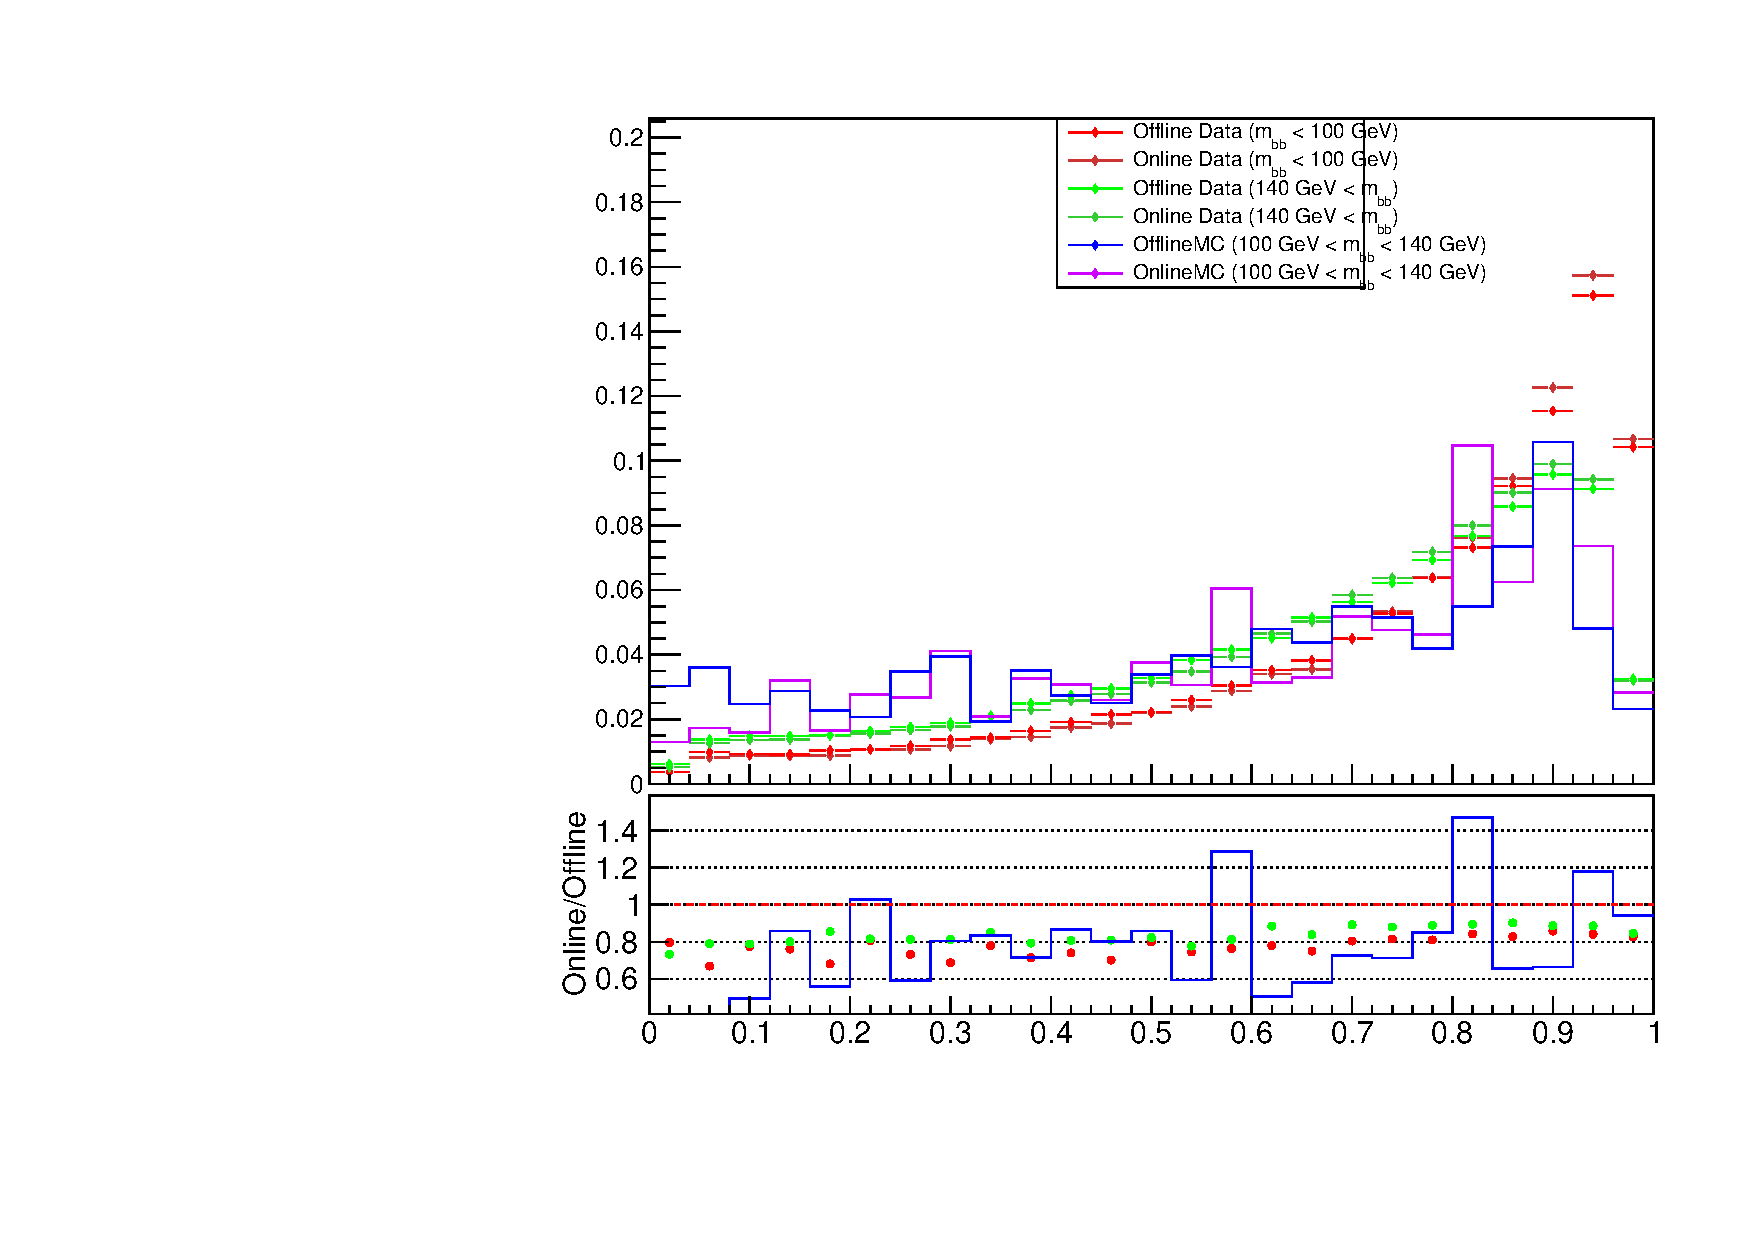
\includegraphics[width=1\linewidth]{ptbalance}
				\caption{}
				\label{fig:bdtptbalance}
			\end{minipage}
		\end{figure}


\section{Mbb Distribution}

		\begin{figure}[h]
			\centering
			\begin{minipage}[h]{0.45\linewidth}
				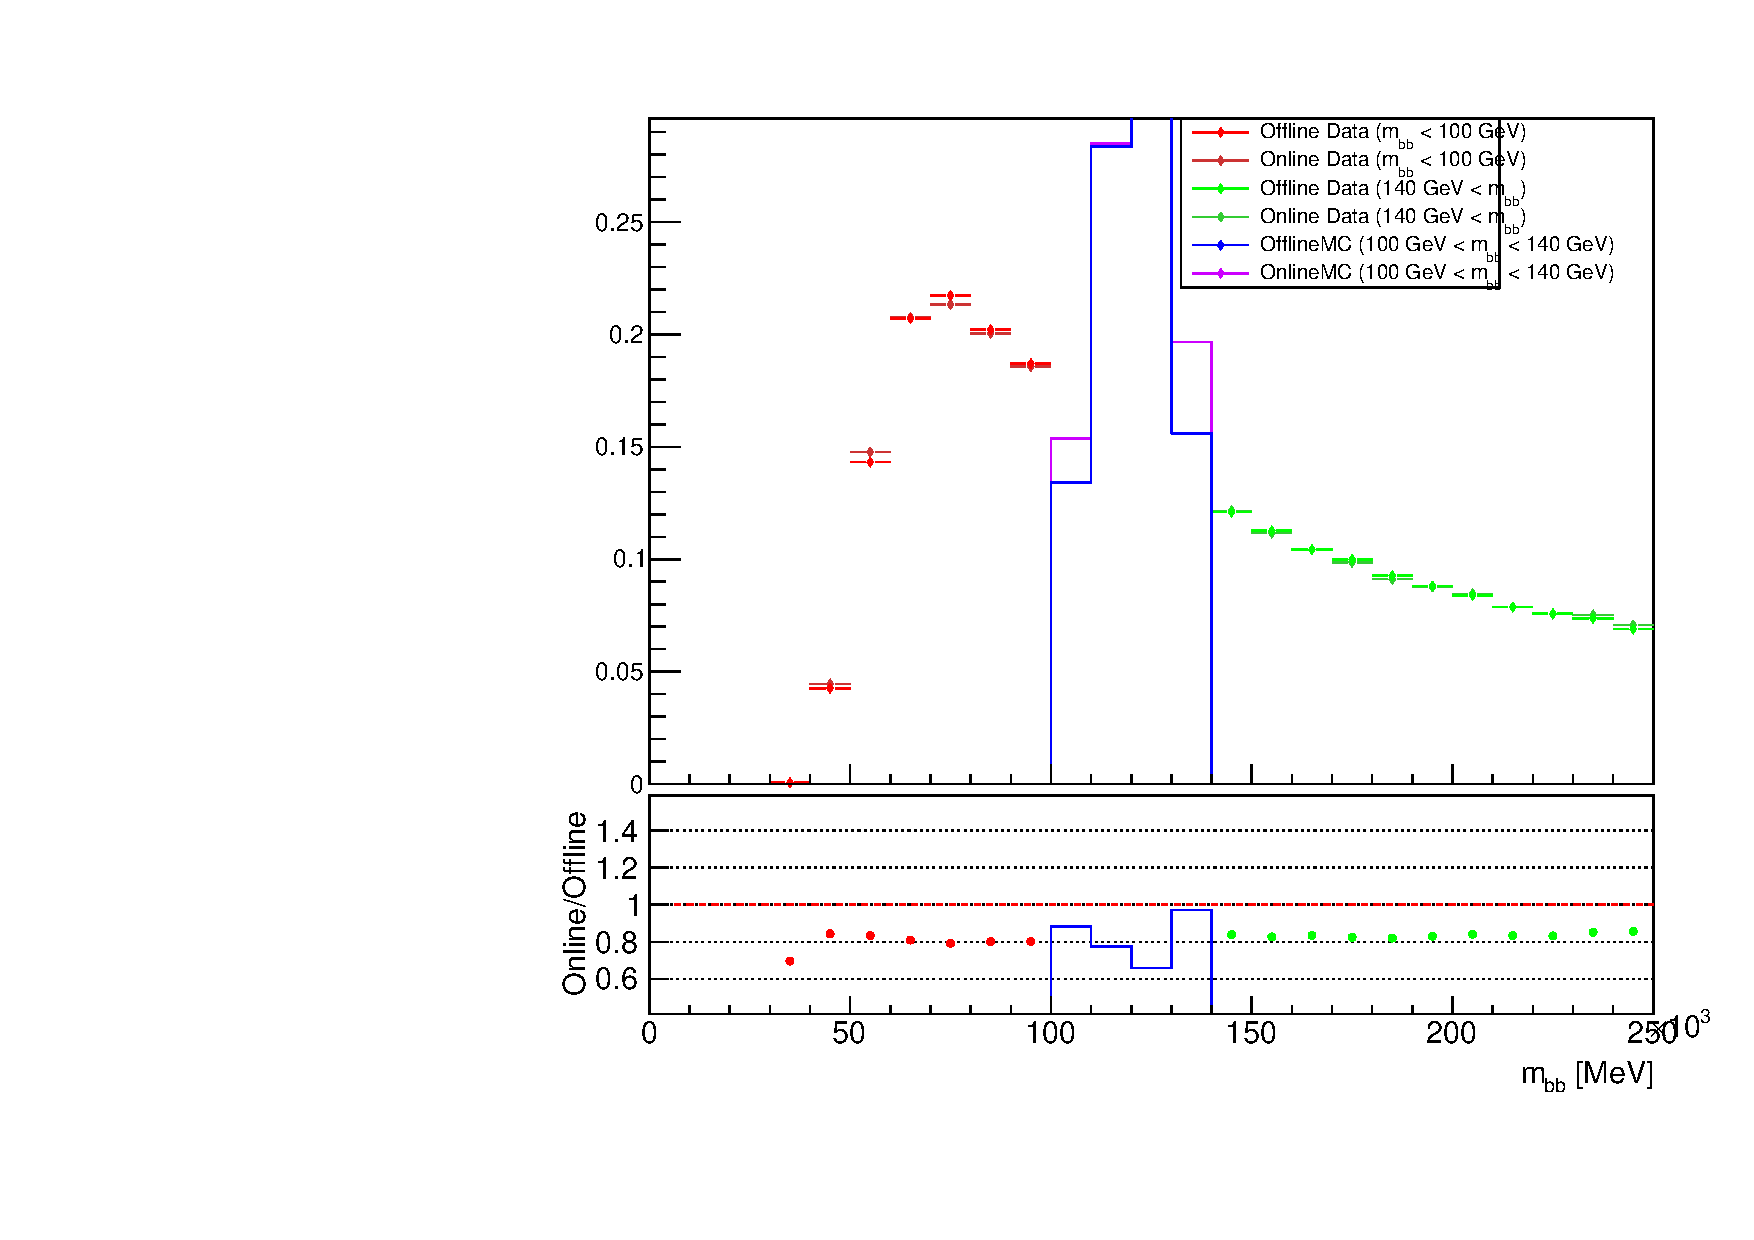
\includegraphics[width=1\linewidth]{mbb}
				\caption{}
				\label{fig:bdtmbb}
			\end{minipage}
			\quad
			\begin{minipage}[h]{0.45\linewidth}
				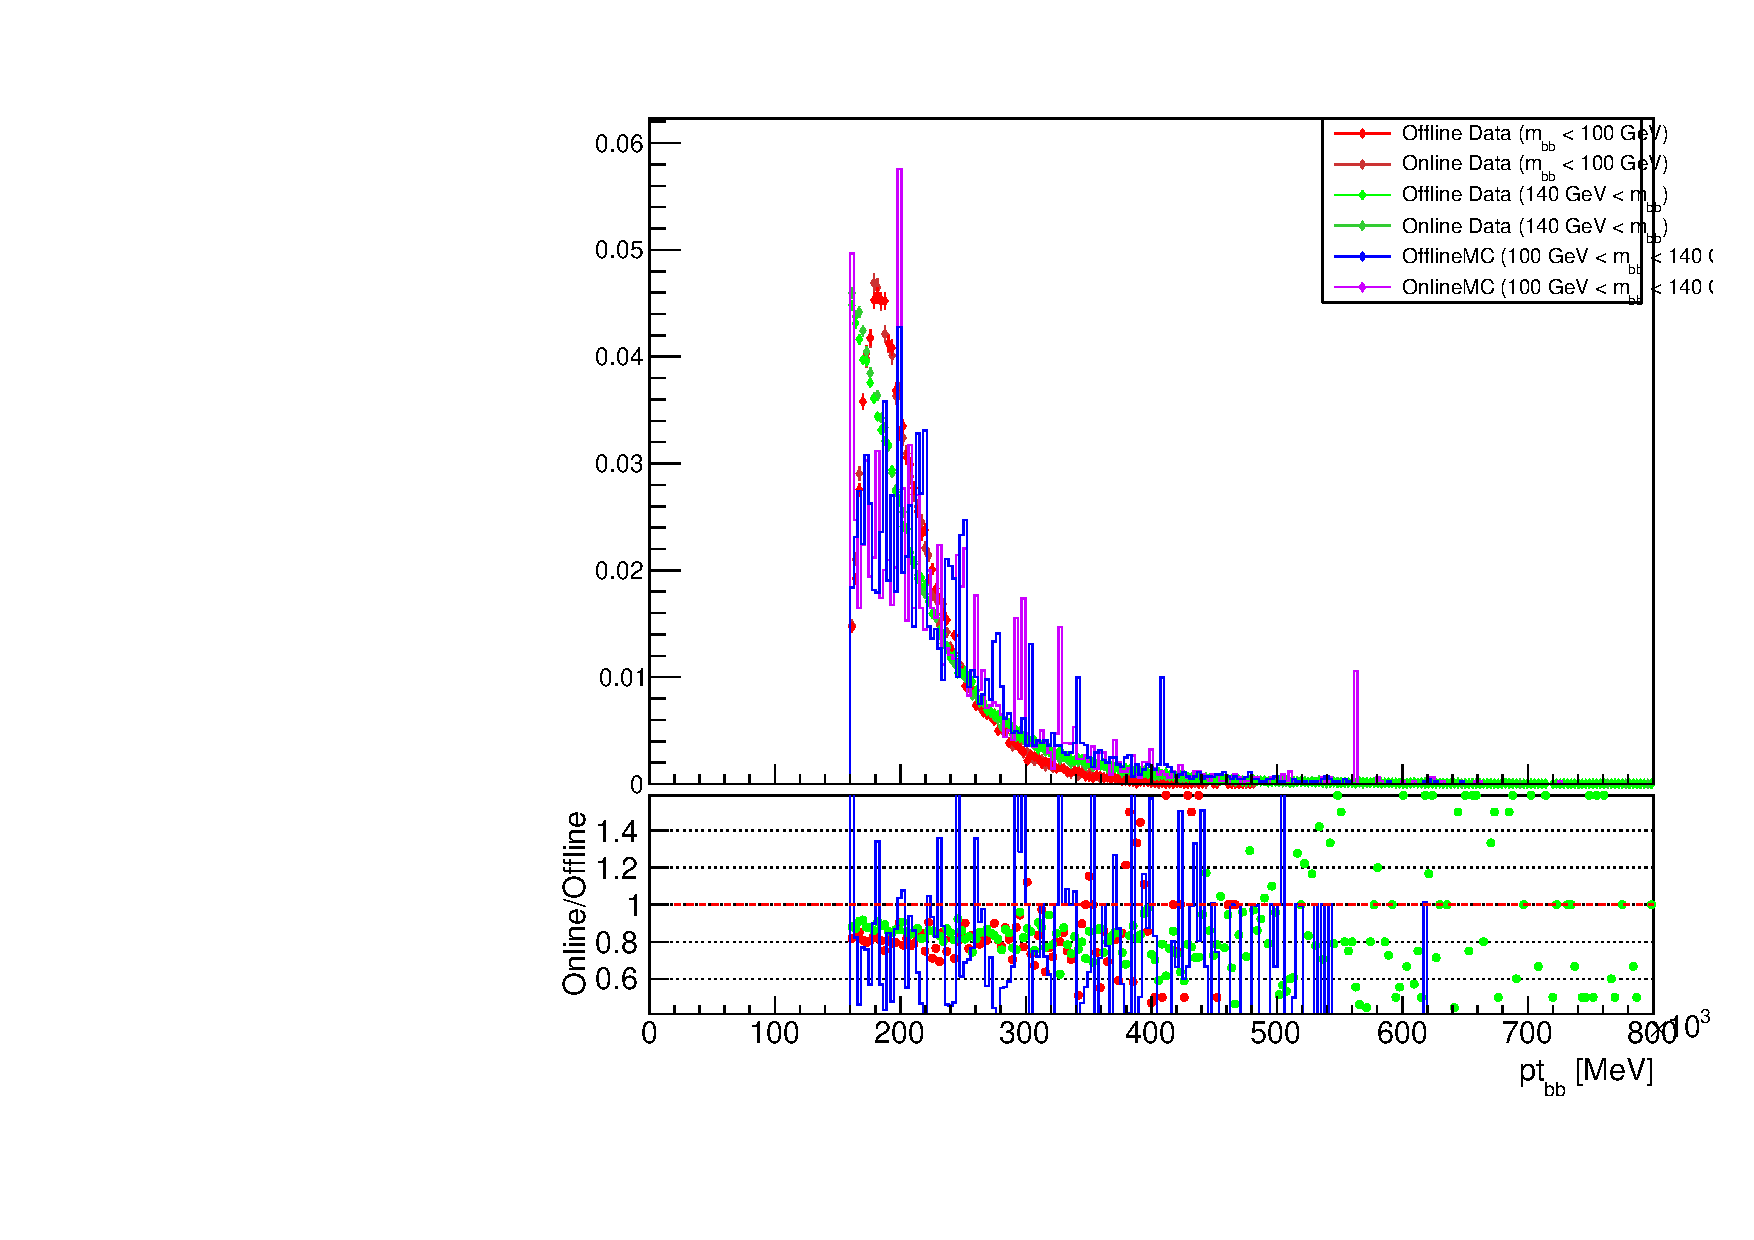
\includegraphics[width=1\linewidth]{ptbb}
				\caption{}
				\label{fig:bdtptbb}
			\end{minipage}
		\end{figure}

	Prior paper suggests this is the 'final' plot, a shape comparison between BDT influenced control and signal regions of the Mbb distribution. A little confused as to exactly what we need here.

\endinput
